\documentclass[12pt]{article}

\usepackage[utf8]{inputenc}
\usepackage[T1]{fontenc}
\usepackage{lmodern}
\usepackage{amsmath,amssymb,mathtools}
\usepackage{booktabs}
\usepackage{longtable}
\usepackage{adjustbox}
\usepackage{array}
\usepackage{graphicx}
\usepackage{float}
\usepackage{caption}
\usepackage{geometry}
\usepackage{parskip}
\usepackage{microtype}
\usepackage{xcolor}
\usepackage[most]{tcolorbox}
\usepackage{enumitem}
\usepackage[round,authoryear]{natbib}
\usepackage{hyperref}

\geometry{a4paper, margin=1in}
\hypersetup{colorlinks=true, linkcolor=black, citecolor=black, urlcolor=black}
\graphicspath{{figures/}}
\captionsetup{font=small,labelfont=bf}

\setlist[itemize]{topsep=3pt,itemsep=2pt,parsep=0pt,leftmargin=1.2cm}
\setlist[enumerate]{topsep=3pt,itemsep=2pt,parsep=0pt,leftmargin=1.2cm}

\newcommand{\Peff}{P_{\mathrm{eff}}}
\newcommand{\Ktot}{K_{\mathrm{tot}}}
\newcommand{\Ksex}{K_{\mathrm{sex}}}
\newcommand{\Kout}{K_{\mathrm{out}}}
\newcommand{\Kbad}{K_{\mathrm{bad}}}
\newcommand{\Rpre}{R^{\mathrm{pre}}}
\newcommand{\Rpost}{R^{\mathrm{post}}}
\newcommand{\E}{\mathbb{E}}
\newcommand{\Var}{\operatorname{Var}}
\newcommand{\sign}{\operatorname{sign}}
\newcommand{\logit}{\operatorname{logit}}
\newcommand{\sech}{\operatorname{sech}}

\newtcolorbox{conclusionbox}[1][]{
  colback=gray!7,
  colframe=black!65,
  title=Conclusion,
  fonttitle=\bfseries,
  sharp corners,
  #1
}

\newtcolorbox{rulebox}[1][]{
  colback=blue!4,
  colframe=black!55,
  title=Rule used,
  fonttitle=\bfseries,
  sharp corners,
  #1
}

\newtcolorbox{cautionbox}[1][]{
  colback=orange!7,
  colframe=black!60,
  title=Caution,
  fonttitle=\bfseries,
  sharp corners,
  #1
}

\newtcolorbox{metaphorbox}[1][]{
  colback=green!5,
  colframe=black!55,
  title=Working metaphor,
  fonttitle=\bfseries,
  sharp corners,
  #1
}

\newtcolorbox{definitionbox}[1][]{
  colback=white,
  colframe=black!55,
  title=Definition,
  fonttitle=\bfseries,
  sharp corners,
  #1
}

\title{Ovule number, pollen competition, and directional reproductive isolation in plants\\[4pt]{\large A theory note, reciprocal-cross audit, and analysis plan}}
\author{Daniel Ortiz-Barrientos\\[3pt]{\normalsize with Kate L. Ostevik, Maddie E. James, and Loren H. Rieseberg}}
\date{\today}

\begin{document}
\maketitle

\begin{abstract}
Here, I develop a model for how post-pollination prezygotic reproductive isolation can arise in flowering plants. The mechanism is the number of effective pollen grains competing per ovule in an ovary. When that ratio is high, pollen grains compete for limited fertilisation opportunities. Selection can then favour pollen traits that win fertilisations and maternal traits that filter pollen more strictly. Reproductive isolation arises as a by-product when the evolved pollen and pistil traits of one lineage no longer work well with those of another. The main empirical prediction is directional. Reciprocal crosses should fail more strongly when the high-competition lineage is the maternal parent. I then audit the current data structure and show that the strongest immediate test is an asymmetric reciprocal-cross test, analysed with family-level partial pooling and sensitivity analyses for ovule-number confidence, genetic distance, mating system, measurement type, and phylogenetic non-independence. The current data support a useful first analysis, but not a fully saturated model.
\end{abstract}

\tableofcontents
\newpage

\section{Purpose of this note}

I want a model that does three jobs. First, it must state the biological mechanism in a testable form. Second, it must show how ovule number, pollen load, mating system, and pollen-pistil mismatch enter the same set of equations. Third, it must lead to predictions that can be separated from older explanations, especially unilateral incompatibility.

The starting idea is simple. An ovary has a finite number of ovules. A stigma receives pollen. If the number of effective pollen grains is smaller than or similar to the number of ovules, most compatible pollen grains can fertilise. Competition among pollen grains is weak. If the number of effective pollen grains is much larger than the number of ovules, some pollen grains must lose. That losing margin creates selection.

\begin{metaphorbox}
Think of ovules as seats in a small room. Pollen grains are applicants for those seats. When there are as many applicants as seats, the filter can be loose. When there are many more applicants than seats, the filter can be strict, and even small differences among applicants matter.
\end{metaphorbox}

The model is not that few ovules directly cause reproductive isolation. The model is that few ovules can move a lineage into a high-competition reproductive state. In that state, selection on pollen performance and maternal filtering becomes stronger. Reproductive isolation can then appear as a passenger of that selection. Ovule number can be thought of as a modulator of the strength of sexual selection in plants. 

\begin{conclusionbox}
The causal claim is not
\[
\hbox{few ovules} \Rightarrow \hbox{reproductive isolation}.
\]
The causal claim is
\begin{align*}
\hbox{few ovules}
&\Rightarrow \hbox{higher pollen competition}\\
&\Rightarrow \hbox{stronger pollen and pistil selection}\\
&\Rightarrow \hbox{directional prezygotic isolation}.
\end{align*}
The middle terms are the mechanism.
\end{conclusionbox}

Note that this model does not predict the evolution of directional postzygotic isolation, a consideration that we explain below. 

\section{Biological background}

Speciation studies often treat reproductive isolation as something that increases with time. This view works well for many postzygotic barriers. Hybrid sterility and hybrid inviability can increase as substitutions accumulate between lineages. In plants, however, post-pollination prezygotic barriers are not only historical residues. They also depend on the current reproductive arena.

After pollen lands on a stigma, it must hydrate, germinate, enter maternal tissues, grow through the style, respond to guidance cues, reach ovules, and release sperm cells. These steps occur inside maternal tissue. They allow selection on pollen traits and on maternal filtering traits (pers. comm. Marcy Uyenoyama, 2007). The pollen tube pathway in angiosperms has therefore been viewed as a setting for pollen competition and selection \citep{Lora2016,LankinenGreen2015}. Reviews of post-pollination barriers also emphasise that pollen-pistil interactions can reject heterospecific pollen and contribute to prezygotic reproductive isolation \citep{WangFilatov2023}.

The important point for this model is that the pistil is not a pipe. It is a selective environment. That environment may become more selective when pollen abundance exceeds ovule abundance.

\begin{conclusionbox}
The pistil is part of the selective environment. This matters because a maternal trait can create a directional barrier. Genetic distance is symmetric. A cross direction is not.
\end{conclusionbox}

\section{Notation}

\begin{center}
\begin{tabular}{>{\raggedright\arraybackslash}p{0.20\linewidth} >{\raggedright\arraybackslash}p{0.72\linewidth}}
\toprule
Symbol & Meaning \\
\midrule
$O_i$ & Number of ovules per ovary in lineage $i$. \\
$A_i$ & Pollen production per relevant unit. The unit must match the biological scale of pollen delivery. \\
$\psi_i$ & Effective deposition fraction. It combines pollen transfer, germination, and timing. \\
$P_{\mathrm{eff},i}$ & Effective pollen load. This is the pollen that can compete for the same ovules. \\
$K_i$ & Effective pollen grains per ovule, $K_i=P_{\mathrm{eff},i}/O_i$. \\
$F_i$ & Strictness of the maternal filter in lineage $i$. \\
$D_{ij}$ & Pollen-pistil mismatch between lineages $i$ and $j$. \\
$G_{ij}$ & Genetic distance or divergence measure between lineages $i$ and $j$. \\
$C_{ii}$ & Conspecific reproductive success for maternal lineage $i$. \\
$H_{i\leftarrow j}$ & Heterospecific reproductive success for cross mother $i$, father $j$. \\
$R_{i\leftarrow j}$ & Directional reproductive isolation index for cross mother $i$, father $j$. \\
$A_{ij}$ & Reciprocal asymmetry, $A_{ij}=R_{i\leftarrow j}-R_{j\leftarrow i}$. \\
$t_i$ & Outcrossing rate of lineage $i$. \\
$s_i$ & Self-incompatibility status of lineage $i$, where $s_i=1$ means SI and $s_i=0$ means SC. \\
\bottomrule
\end{tabular}
\end{center}

\section{The competition ratio}

\subsection{Definition}

The central quantity is
\begin{equation}
K_i = \frac{P_{\mathrm{eff},i}}{O_i}.
\label{eq:Kdef}
\end{equation}
Here $P_{\mathrm{eff},i}$ is not total pollen production. It is not even necessarily the total pollen counted on the stigma. It is the pollen that can plausibly compete for the same ovules. A pollen grain contributes to $P_{\mathrm{eff},i}$ only if it arrives in the relevant time window, remains viable, germinates, and enters the competitive pathway.

\begin{definitionbox}
$K_i$ is the number of effective pollen grains per ovule. It is a competition index, not a pollen count.
\end{definitionbox}

A useful decomposition is
\begin{equation}
P_{\mathrm{eff},i} = \psi_i A_i,
\label{eq:PeffPsiA}
\end{equation}
where $A_i$ is pollen production and $\psi_i$ is the effective deposition fraction. We can write
\begin{equation}
\psi_i = \delta_i \gamma_i \tau_i.
\label{eq:psi}
\end{equation}
Here $\delta_i$ is the fraction of produced pollen that reaches a focal stigma, $\gamma_i$ is the fraction of deposited pollen that germinates or enters the pollen-tube pool, and $\tau_i$ measures temporal overlap among competing pollen grains.

Substituting \eqref{eq:PeffPsiA} into \eqref{eq:Kdef} gives
\begin{equation}
K_i = \frac{\psi_i A_i}{O_i}.
\label{eq:KpsiA}
\end{equation}

\begin{cautionbox}
A fixed pollen-deposition fraction, such as $\psi=0.02$, is useful for simulation. It should not be treated as a biological constant. It is a calibration value.
\end{cautionbox}

\subsection{Why the ratio matters}

When $K_i \leq 1$, the effective pollen load is no larger than the ovule number. Pollen may still fail for physiological reasons, but there is little numerical pressure for pollen grains to exclude one another.

When $K_i>1$, the effective pollen load exceeds the number of ovules. Only a subset of pollen grains can fertilise. This creates the opportunity for selection among pollen grains.

One simple index of that opportunity is
\begin{equation}
\Omega_i=
\E\left[\frac{(P_{if}-O_i)_+}{P_{if}}\right],
\label{eq:Omega}
\end{equation}
where $P_{if}$ is the effective pollen load on flower $f$ and
\begin{equation}
(x)_+=\begin{cases}
x, & x>0,\\
0, & x\leq 0.
\end{cases}
\end{equation}
The numerator $P_{if}-O_i$ is the number of pollen grains that cannot win an ovule when pollen exceeds ovules. The denominator $P_{if}$ turns that number into a fraction.

\begin{conclusionbox}
$K$ says whether competition is possible on average. $\Omega$ says how much pollen is excluded at the flower level. Both quantities should be high in the strongest version of the model.
\end{conclusionbox}

\section{Sublinear pollen-load scaling}

The model needs one scaling condition. Effective pollen load should increase with ovule number more slowly than one-to-one. Write
\begin{equation}
P_{\mathrm{eff},i} = \psi c O_i^\alpha,
\label{eq:sublinear}
\end{equation}
where $c>0$ and $\alpha$ is the scaling exponent.

Substitute \eqref{eq:sublinear} into the definition of $K_i$:
\begin{align}
K_i
&=\frac{P_{\mathrm{eff},i}}{O_i} \\
&=\frac{\psi c O_i^\alpha}{O_i}. 
\end{align}

Now use the exponent rule
\begin{equation}
\frac{O_i^\alpha}{O_i}=\frac{O_i^\alpha}{O_i^1}=O_i^{\alpha-1}.
\end{equation}
Therefore
\begin{equation}
K_i=\psi c O_i^{\alpha-1}.
\label{eq:Ksublinear}
\end{equation}

\begin{rulebox}
The exponent rule used above is
\[
\frac{x^a}{x^b}=x^{a-b}.
\]
Here $a=\alpha$ and $b=1$.
\end{rulebox}

Take logs of both sides of \eqref{eq:Ksublinear}:
\begin{align}
\log K_i
&=\log(\psi c O_i^{\alpha-1}) \\
&=\log \psi + \log c + \log(O_i^{\alpha-1}) \\
&=\log(\psi c) + (\alpha-1)\log O_i.
\label{eq:logK}
\end{align}

Differentiate \eqref{eq:logK} with respect to $\log O_i$:
\begin{equation}
\frac{\partial \log K_i}{\partial \log O_i}=\alpha-1.
\label{eq:dlogKdlogO}
\end{equation}

If $\alpha<1$, then $\alpha-1<0$. Thus
\begin{equation}
\frac{\partial \log K_i}{\partial \log O_i}<0.
\end{equation}

\begin{conclusionbox}
If effective pollen load scales sublinearly with ovule number, then the pollen-per-ovule ratio declines as ovule number rises. Few-ovule lineages have the stronger competition regime.
\end{conclusionbox}

\subsection{The competition threshold}

The threshold between weak and strong numerical competition is $K_i=1$. Use \eqref{eq:Ksublinear}:
\begin{equation}
1=\psi c O_i^{\alpha-1}.
\end{equation}
Move $\psi c$ to the left-hand side:
\begin{equation}
\frac{1}{\psi c}=O_i^{\alpha-1}.
\end{equation}
Because $\alpha-1=-(1-\alpha)$, we can write
\begin{equation}
O_i^{\alpha-1}=O_i^{-(1-\alpha)}=\frac{1}{O_i^{1-\alpha}}.
\end{equation}
Thus
\begin{equation}
\frac{1}{\psi c}=\frac{1}{O_i^{1-\alpha}}.
\end{equation}
Invert both sides:
\begin{equation}
\psi c = O_i^{1-\alpha}.
\end{equation}
Raise both sides to the power $1/(1-\alpha)$:
\begin{equation}
O^*=(\psi c)^{1/(1-\alpha)}.
\label{eq:Ostar}
\end{equation}

\begin{conclusionbox}
There is no universal ovule threshold. The threshold depends on pollen production, pollen transfer, germination, timing, and the scaling exponent $\alpha$.
\end{conclusionbox}

\section{Selection among pollen grains}

\subsection{Saved fraction}

Assume a flower receives $P$ effective pollen grains and has $O$ ovules. If $P>O$, then only $O$ pollen grains can win. The fraction of pollen grains that win is
\begin{equation}
q=\frac{O}{P}.
\end{equation}
Since $K=P/O$, we have $P=KO$. Substitute this into the equation for $q$:
\begin{align}
q&=\frac{O}{KO} \\
&=\frac{1}{K}.
\label{eq:q}
\end{align}

\begin{conclusionbox}
When $K=2$, half the pollen grains can win. When $K=10$, one tenth can win. As $K$ rises, the winners come from a smaller and more extreme part of the pollen-performance distribution.
\end{conclusionbox}

\subsection{Truncation selection}

Let $z$ be pollen competitive performance. This could represent pollen-tube growth rate, success in maternal tissue, response to ovule guidance, or a weighted combination of such traits. For the first derivation, assume
\begin{equation}
z\sim N(\bar{z},\sigma_z^2).
\end{equation}
We can standardise $z$ as
\begin{equation}
x=\frac{z-\bar{z}}{\sigma_z},
\end{equation}
so that
\begin{equation}
x\sim N(0,1).
\end{equation}

If only the top fraction $q$ of pollen grains succeeds, then the cutoff on the standard normal scale is
\begin{equation}
t=\Phi^{-1}(1-q),
\end{equation}
where $\Phi^{-1}$ is the standard normal quantile function.

The mean of a standard normal variable above cutoff $t$ is
\begin{equation}
\E[x\mid x>t]=\frac{\phi(t)}{1-\Phi(t)}.
\end{equation}
But $1-\Phi(t)=q$. Therefore
\begin{equation}
\E[x\mid x>t]=\frac{\phi(t)}{q}.
\end{equation}
Return to the original scale. Since $z=\bar{z}+\sigma_z x$,
\begin{equation}
\E[z\mid z>z_t]=\bar{z}+\sigma_z\frac{\phi(t)}{q}.
\end{equation}
The selection differential is the mean of successful pollen minus the original mean:
\begin{align}
S_z
&=\E[z\mid z>z_t]-\bar{z} \\
&=\sigma_z\frac{\phi(t)}{q}.
\end{align}
Now use $q=1/K$ from \eqref{eq:q}. Then
\begin{equation}
t=\Phi^{-1}\left(1-\frac{1}{K}\right),
\end{equation}
and
\begin{equation}
S_z(K)=\sigma_z K\phi\left[\Phi^{-1}\left(1-\frac{1}{K}\right)\right]
\quad \hbox{for } K>1.
\end{equation}
Set $S_z(K)=0$ for $K\leq 1$. The full expression is
\begin{equation}
S_z(K)=
\begin{cases}
0, & K\leq 1,\\[6pt]
\sigma_z K\phi\left[\Phi^{-1}\left(1-\dfrac{1}{K}\right)\right], & K>1.
\end{cases}
\label{eq:Sz}
\end{equation}

\begin{rulebox}
The calculation uses the mean of a truncated normal distribution. For a standard normal variable $x$, the mean above cutoff $t$ is
\[
\E[x\mid x>t]=\frac{\phi(t)}{1-\Phi(t)}.
\]
The denominator is the saved fraction.
\end{rulebox}

\subsection{From selection differential to allele-frequency change}

The selection gradient on pollen performance is
\begin{equation}
\beta_z(K)=\frac{S_z(K)}{\sigma_z^2}.
\label{eq:betaz}
\end{equation}
This says how much relative success changes per unit of pollen performance.

Let allele $\ell$ increase pollen performance by $a_\ell$. A first-order approximation to its male-function selection coefficient is
\begin{equation}
s_{\ell}^{(m)}(K)\approx a_\ell\beta_z(K).
\end{equation}
If only part of the pollen-phase advantage is expressed in whole-plant allele-frequency change, write
\begin{equation}
s_{\ell}^{\mathrm{eff}}(K)=\kappa a_\ell\beta_z(K),
\label{eq:seff}
\end{equation}
where $0<\kappa\leq 1$.

For an allele at frequency $p_\ell$, the standard weak-selection recursion is
\begin{equation}
\Delta p_\ell\approx p_\ell(1-p_\ell)s_{\ell}^{\mathrm{eff}}(K).
\label{eq:deltap}
\end{equation}
Substitute \eqref{eq:seff}:
\begin{equation}
\Delta p_\ell\approx p_\ell(1-p_\ell)\kappa a_\ell\beta_z(K).
\end{equation}
Now substitute $K=\psi cO^{\alpha-1}$:
\begin{equation}
\Delta p_\ell\approx p_\ell(1-p_\ell)\kappa a_\ell
\beta_z\left(\psi cO^{\alpha-1}\right).
\label{eq:deltapO}
\end{equation}

\begin{conclusionbox}
If $\alpha<1$, then lower ovule number increases $K$. Higher $K$ increases the truncation-selection differential. Thus few-ovule lineages should experience stronger selection on pollen-performance alleles, all else equal.
\end{conclusionbox}

\section{Maternal filtering}

Selection among pollen grains can change male function. Directional reproductive isolation also needs a maternal component. Let $F_i\geq 0$ be the strictness of the maternal filter in lineage $i$.

A strict filter has two effects. It can improve offspring quality by rejecting unsuitable pollen. It can also reduce seed set when pollen is scarce. The balance between these effects depends on $K$.

\subsection{A simple fitness model for the filter}

Let the accepted fraction of pollen decline with filter strictness as $e^{-F}$. Then the accepted pollen-per-ovule ratio is
\begin{equation}
Ke^{-F}.
\end{equation}
Use a saturating seed-set function:
\begin{equation}
S(K,F)=1-e^{-Ke^{-F}}.
\label{eq:seedset}
\end{equation}
This function is near zero when accepted pollen is scarce. It approaches one when accepted pollen is abundant.

Let the offspring-quality benefit of filtering be
\begin{equation}
Q(F)=1+b(1-e^{-\lambda F}),
\label{eq:quality}
\end{equation}
where $b>0$ is the maximum quality benefit and $\lambda>0$ controls how fast the benefit rises.

Let the direct cost of strictness be
\begin{equation}
C(F)=e^{-c_FF^2/2},
\label{eq:cost}
\end{equation}
where $c_F>0$.

Maternal fitness is
\begin{equation}
W_f(F,K)=S(K,F)Q(F)C(F).
\label{eq:Wfilter}
\end{equation}

Take logs because products become sums:
\begin{equation}
\log W_f(F,K)=\log S(K,F)+\log Q(F)-\frac{c_FF^2}{2}.
\label{eq:logWfilter}
\end{equation}

\begin{rulebox}
Maximising $W$ is equivalent to maximising $\log W$ when $W>0$, because the log function is monotonic. We use logs because derivatives of sums are easier than derivatives of products.
\end{rulebox}

\subsection{The first-order condition}

The optimum filter $F^*(K)$ solves
\begin{equation}
\frac{\partial \log W_f(F,K)}{\partial F}=0.
\end{equation}
We now compute each term.

First, define
\begin{equation}
x=Ke^{-F}.
\end{equation}
Then $S(K,F)=1-e^{-x}$. The derivative of $x$ with respect to $F$ is
\begin{equation}
\frac{\partial x}{\partial F}=-Ke^{-F}=-x.
\end{equation}
The derivative of $S$ with respect to $F$ is
\begin{align}
\frac{\partial S}{\partial F}
&=\frac{\partial}{\partial F}(1-e^{-x}) \\
&=e^{-x}\frac{\partial x}{\partial F} \\
&=-xe^{-x}.
\end{align}
Therefore
\begin{equation}
\frac{\partial \log S}{\partial F}
=\frac{1}{S}\frac{\partial S}{\partial F}
=-\frac{xe^{-x}}{1-e^{-x}}.
\label{eq:dlogS}
\end{equation}

Second, for $Q(F)=1+b(1-e^{-\lambda F})$,
\begin{equation}
\frac{\partial Q}{\partial F}=b\lambda e^{-\lambda F}.
\end{equation}
Thus
\begin{equation}
\frac{\partial \log Q}{\partial F}=
\frac{b\lambda e^{-\lambda F}}{1+b(1-e^{-\lambda F})}.
\label{eq:dlogQ}
\end{equation}

Third,
\begin{equation}
\frac{\partial}{\partial F}\left(-\frac{c_FF^2}{2}\right)=-c_FF.
\label{eq:dcost}
\end{equation}

Combine \eqref{eq:dlogS}, \eqref{eq:dlogQ}, and \eqref{eq:dcost}. The optimum satisfies
\begin{equation}
-\frac{xe^{-x}}{1-e^{-x}}
+
\frac{b\lambda e^{-\lambda F}}{1+b(1-e^{-\lambda F})}
-c_FF=0,
\quad x=Ke^{-F}.
\label{eq:FOCfilter}
\end{equation}

The first term is the seed-set cost of filtering. It is negative. The second term is the offspring-quality benefit of filtering. It is positive. The third term is the direct cost of filter strictness. It is negative.

As $K$ rises, $x=Ke^{-F}$ rises at any fixed $F$. The magnitude of the seed-set cost term
\begin{equation}
\frac{xe^{-x}}{1-e^{-x}}=\frac{x}{e^x-1}
\end{equation}
declines as $x$ increases. This means pollen surplus makes filtering cheaper. The optimum filter therefore shifts upward over the parameter range where filtering gives a quality benefit.

\begin{conclusionbox}
High $K$ does not make a strict pistil inevitable. It makes a strict pistil cheaper. If filtering improves offspring quality or avoids poor pollen, selection can then favour a higher $F$ (pers. comm. John Willis and Marcy Uyenoyama, 2007).
\end{conclusionbox}

For the rest of the model we use the qualitative result
\begin{equation}
\frac{dF^*(K)}{dK}>0.
\label{eq:dFdK}
\end{equation}

\section{Mating system as a modifier of competition}

Mating system changes what $K$ means. A selfing plant can place many pollen grains on its own stigma. That may produce a high total pollen-per-ovule ratio. But if the pollen comes from one genotype, the opportunity for sexual selection among paternal genotypes is limited.

We therefore distinguish total pollen competition from genetically diverse pollen competition.

\subsection{Partitioning the pollen pool}

Write the effective pollen load as
\begin{equation}
P_{\mathrm{eff},i}=P_{s,i}+P_{x,i}+P_{h,i},
\label{eq:pollenpartition}
\end{equation}
where $P_{s,i}$ is self pollen, $P_{x,i}$ is conspecific outcross pollen, and $P_{h,i}$ is heterospecific pollen.

The total competition ratio is
\begin{equation}
K_{\mathrm{tot},i}=\frac{P_{s,i}+P_{x,i}+P_{h,i}}{O_i}.
\label{eq:Ktot}
\end{equation}
The outcross competition ratio is
\begin{equation}
K_{\mathrm{out},i}=\frac{P_{x,i}}{O_i}.
\label{eq:Kout}
\end{equation}
The costly-pollen ratio is
\begin{equation}
K_{\mathrm{bad},i}=\frac{P_{s,i}+P_{h,i}}{O_i}.
\label{eq:Kbad}
\end{equation}
Here ``bad'' means costly in the context of maternal fitness. Self pollen can be costly if inbreeding depression is high. Heterospecific pollen can be costly if it blocks conspecific fertilisation, creates inviable seeds, or wastes ovules.

Now define pollen donor diversity. Let $\pi_{ig}$ be the fraction of the effective pollen pool on lineage $i$ contributed by donor genotype $g$. A simple diversity index is
\begin{equation}
D^{\mathrm{pollen}}_i=1-\sum_g \pi_{ig}^2.
\label{eq:pollenDiversity}
\end{equation}
This is close to zero when most effective pollen comes from one genotype. It is larger when many donors contribute.

Define sexually effective competition as
\begin{equation}
K_{\mathrm{sex},i}=K_{\mathrm{tot},i}D^{\mathrm{pollen}}_i.
\label{eq:Ksex}
\end{equation}

\begin{conclusionbox}
The model should use $\Ksex$, not only $\Ktot$, when the question is sexual selection among genetically distinct pollen donors. Total pollen can be high in selfers, while sexually effective competition remains low.
\end{conclusionbox}

\subsection{Expected mating-system regimes}

The ovule-gated signal should be strongest in lineages where surplus pollen is also genetically diverse. That points to outcrossers and mixed-maters, not predominant autonomous selfers.

\begin{center}
\begin{tabular}{>{\raggedright\arraybackslash}p{0.25\linewidth} >{\raggedright\arraybackslash}p{0.32\linewidth} >{\raggedright\arraybackslash}p{0.32\linewidth}}
\toprule
Mating system & Effect on $K$ & Expected ovule-gated signal \\
\midrule
Obligate outcrossing or strong self-incompatibility & High donor diversity if pollen is abundant. Self pollen is rejected or ineffective. & Strong, but SI itself can confound maternal rejection. \\
Mostly outcrossing and self-compatible & High outcross pollen with some self pollen. & Strong if outcross pollen is abundant and donor diversity is high. \\
Mixed mating with competing selfing & Self and outcross pollen arrive in the same window. & Strong. This is a good regime for cryptic maternal filtering. \\
Mixed mating with delayed selfing & Outcross pollen has the first chance; selfing provides backup. & Moderate to strong. The timing helps preserve outcross competition. \\
Predominant autonomous selfing & Total pollen can be high, but donor diversity is low. & Weak or absent for this mechanism. RI may evolve through other routes. \\
\bottomrule
\end{tabular}
\end{center}

\begin{metaphorbox}
Mating system is a valve. Ovule number sets the number of seats. Pollen production sets the number of applicants. The mating system controls whether the applicants are genetically distinct or mostly copies of the same donor.
\end{metaphorbox}

\subsection{A maternal-filter model with self and outcross pollen}

A maternal filter should be favoured when there is enough acceptable pollen to replace rejected pollen and enough costly pollen to make rejection useful. One way to write this is
\begin{equation}
W_i(F)=
\left[1-\exp\left(-\frac{P_{x,i}+e^{-F_s}P_{s,i}+e^{-F_h}P_{h,i}}{O_i}\right)\right]
\left[1-\delta_i
\frac{e^{-F_s}P_{s,i}}{P_{x,i}+e^{-F_s}P_{s,i}+e^{-F_h}P_{h,i}}\right]
\exp\left(-\frac{c_FF^2}{2}\right).
\label{eq:Wmating}
\end{equation}
Here $F_s$ is filtering against self pollen, $F_h$ is filtering against heterospecific pollen, and $\delta_i$ is inbreeding depression.

The first bracket is seed-set assurance. The second bracket is offspring-quality protection against selfed progeny. The final term is the cost of filter strictness. The equation can be simplified in simulations, but it states the logic.

\begin{conclusionbox}
Strict maternal filtering is most likely when three conditions hold: outcross pollen is abundant, costly pollen is also present, and the fitness cost of accepting costly pollen is high.
\end{conclusionbox}

\subsection{Regression form with mating system}

If $K$ is measured or estimated, the empirical model for directed prezygotic success can include an interaction between maternal competition and outcrossing:
\begin{equation}
\logit\left(p^{\mathrm{pre}}_{i\leftarrow j}\right)
=
\beta_0+\beta_K\log K_i+\beta_t t_i+\beta_{Kt}\log K_i\,t_i+\beta_GG_{ij}+\cdots.
\label{eq:matingRegression}
\end{equation}
Here $t_i$ is the outcrossing rate of the maternal lineage. The key coefficient is $\beta_{Kt}$.

For asymmetry, use
\begin{equation}
A_{ij}=\beta_0+\beta_1\left[G_{ij}(\log O_j-\log O_i)\right]
+\beta_2\bar{t}_{ij}\left[G_{ij}(\log O_j-\log O_i)\right]
+\epsilon_{ij},
\label{eq:matingAsymmetry}
\end{equation}
where $\bar{t}_{ij}=(t_i+t_j)/2$. The prediction is that the ovule-gated effect should be stronger when $\bar{t}_{ij}$ is high.

\begin{cautionbox}
Do not pool selfers, mixed-maters, and outcrossers without modelling mating system. A weak pooled signal could mean the mechanism is absent. It could also mean the mechanism is present only where genetically diverse pollen competition exists.
\end{cautionbox}

\section{Prezygotic reproductive isolation}

\subsection{The reproductive isolation index}

For the directed cross mother $i$, father $j$, let $C_{ii}$ be the conspecific reproductive success of maternal lineage $i$. Let $H_{i\leftarrow j}$ be the heterospecific success when lineage $i$ provides the ovules and lineage $j$ provides pollen.

Use the Sobel--Chen index \citep{SobelChen2014}:
\begin{equation}
R_{i\leftarrow j}=1-\frac{2H_{i\leftarrow j}}{H_{i\leftarrow j}+C_{ii}}.
\label{eq:SobelChen}
\end{equation}
Define the relative heterospecific success
\begin{equation}
h_{i\leftarrow j}=\frac{H_{i\leftarrow j}}{C_{ii}}.
\label{eq:hdef}
\end{equation}
This compares the heterospecific cross with the mother's own conspecific baseline.

Now derive the simplified form. From \eqref{eq:hdef},
\begin{equation}
H_{i\leftarrow j}=h_{i\leftarrow j}C_{ii}.
\end{equation}
Substitute this into \eqref{eq:SobelChen}:
\begin{align}
R_{i\leftarrow j}
&=1-\frac{2h_{i\leftarrow j}C_{ii}}{h_{i\leftarrow j}C_{ii}+C_{ii}} \\
&=1-\frac{2h_{i\leftarrow j}C_{ii}}{C_{ii}(h_{i\leftarrow j}+1)} \\
&=1-\frac{2h_{i\leftarrow j}}{1+h_{i\leftarrow j}} \\
&=\frac{1+h_{i\leftarrow j}}{1+h_{i\leftarrow j}}-\frac{2h_{i\leftarrow j}}{1+h_{i\leftarrow j}} \\
&=\frac{1-h_{i\leftarrow j}}{1+h_{i\leftarrow j}}.
\end{align}
Thus
\begin{equation}
\boxed{R_{i\leftarrow j}=\frac{1-h_{i\leftarrow j}}{1+h_{i\leftarrow j}}}.
\label{eq:Rh}
\end{equation}

\begin{conclusionbox}
The index depends on heterospecific success relative to the mother's own baseline. This is important. It prevents a low-fecundity mother from appearing isolated simply because she has low success in all crosses.
\end{conclusionbox}

\subsection{Mechanistic content of relative success}

The ovule-gated model puts the maternal filter into $h_{i\leftarrow j}$. Let $D_{ij}$ be the mismatch between the pollen-pistil systems of lineages $i$ and $j$. Start with a symmetric mismatch:
\begin{equation}
D_{ij}=D_{ji}.
\end{equation}
The directed part is the maternal filter $F_i$. Write
\begin{equation}
h_{i\leftarrow j}=\exp(-F_iD_{ij}).
\label{eq:hfilter}
\end{equation}

This equation has three assumptions.

\begin{enumerate}
\item Mismatch is a property of the pair: $D_{ij}=D_{ji}$.
\item Conspecific mismatch is zero: $D_{ii}=0$.
\item Filter strictness is a property of the mother: $F_i=F^*(K_i)$.
\end{enumerate}

If a strict filter also lowers conspecific success, some of its effect will cancel when we normalise by $C_{ii}$. That case is biologically possible. The model should treat it as a sensitivity analysis.

Substitute \eqref{eq:hfilter} into \eqref{eq:Rh}:
\begin{equation}
R_{i\leftarrow j}=\frac{1-e^{-F_iD_{ij}}}{1+e^{-F_iD_{ij}}}.
\label{eq:Rfilter}
\end{equation}
This expression can be written as a hyperbolic tangent:
\begin{equation}
R_{i\leftarrow j}=\tanh\left(\frac{F_iD_{ij}}{2}\right).
\label{eq:tanhR}
\end{equation}

\begin{rulebox}
The identity used above is
\[
\tanh(x/2)=\frac{1-e^{-x}}{1+e^{-x}}.
\]
Here $x=F_iD_{ij}$.
\end{rulebox}

\section{Directional asymmetry}

\subsection{Exact expression}

Define reciprocal asymmetry as
\begin{equation}
A_{ij}=R_{i\leftarrow j}-R_{j\leftarrow i}.
\label{eq:Adef}
\end{equation}
Using \eqref{eq:tanhR},
\begin{equation}
A_{ij}=\tanh\left(\frac{F_iD_{ij}}{2}\right)
-
\tanh\left(\frac{F_jD_{ij}}{2}\right).
\label{eq:Aexact}
\end{equation}
This is the exact asymmetry under the model.

\subsection{The sign theorem}

The function $\tanh(x)$ is strictly increasing. If $D_{ij}>0$, then
\begin{equation}
F_i>F_j
\quad \Rightarrow \quad
\frac{F_iD_{ij}}{2}>\frac{F_jD_{ij}}{2}.
\end{equation}
Because $\tanh$ is increasing,
\begin{equation}
\tanh\left(\frac{F_iD_{ij}}{2}\right)>
\tanh\left(\frac{F_jD_{ij}}{2}\right).
\end{equation}
Therefore
\begin{equation}
A_{ij}>0.
\end{equation}
The same reasoning gives
\begin{equation}
\boxed{\sign(A_{ij})=\sign(F_i-F_j)}.
\label{eq:sign}
\end{equation}

\begin{conclusionbox}
Symmetric divergence can build a barrier, but it cannot choose a cross direction. Directional asymmetry requires a directional trait. In this model that trait is the maternal filter.
\end{conclusionbox}

\subsection{Small-mismatch approximation}

For small $x$,
\begin{equation}
\tanh(x)\approx x.
\end{equation}
In \eqref{eq:tanhR}, $x=F_iD_{ij}/2$. Therefore
\begin{equation}
R_{i\leftarrow j}\approx \frac{F_iD_{ij}}{2}.
\label{eq:Rlin}
\end{equation}
Apply this to both reciprocal directions:
\begin{align}
R_{i\leftarrow j}&\approx \frac{F_iD_{ij}}{2},\\
R_{j\leftarrow i}&\approx \frac{F_jD_{ij}}{2}.
\end{align}
Subtract:
\begin{align}
A_{ij}
&=R_{i\leftarrow j}-R_{j\leftarrow i} \\
&\approx \frac{F_iD_{ij}}{2}-\frac{F_jD_{ij}}{2} \\
&=\frac{D_{ij}}{2}(F_i-F_j).
\end{align}
Thus
\begin{equation}
\boxed{A_{ij}\approx \frac{1}{2}D_{ij}(F_i-F_j)}.
\label{eq:Alin}
\end{equation}

\begin{conclusionbox}
The factor $1/2$ comes from the Sobel--Chen index. A simpler $1-C$ index would not have this factor.
\end{conclusionbox}

\subsection{From filter strictness to ovule number}

We now connect $F_i-F_j$ to ovule number. The chain is
\begin{equation}
O_i \rightarrow K_i \rightarrow F_i.
\end{equation}
From \eqref{eq:Ksublinear},
\begin{equation}
K_i=\psi cO_i^{\alpha-1}.
\end{equation}
Using \eqref{eq:dFdK}, $F$ increases with $K$. We need the derivative of $F$ with respect to $\log O$.

Use the chain rule:
\begin{equation}
\frac{dF}{d\log O}=\frac{dF}{dK}\frac{dK}{d\log O}.
\end{equation}
We now compute $dK/d\log O$. Since
\begin{equation}
\log K=\log(\psi c)+(\alpha-1)\log O,
\end{equation}
we have
\begin{equation}
\frac{d\log K}{d\log O}=\alpha-1.
\end{equation}
For any positive variable $K$,
\begin{equation}
\frac{dK}{d\log O}=K\frac{d\log K}{d\log O}.
\end{equation}
Therefore
\begin{equation}
\frac{dK}{d\log O}=K(\alpha-1).
\end{equation}
So
\begin{equation}
\frac{dF}{d\log O}=F'(K)K(\alpha-1).
\label{eq:dFdlogO}
\end{equation}
Because $F'(K)>0$ and $\alpha<1$, this derivative is negative.

Define the positive sensitivity
\begin{equation}
\beta_F=-\frac{dF}{d\log O}=F'(K)K(1-\alpha)>0.
\label{eq:betaF}
\end{equation}
Then a first-order approximation gives
\begin{equation}
F_i-F_j\approx \beta_F(\log O_j-\log O_i).
\label{eq:FdiffOdiff}
\end{equation}

\begin{rulebox}
The sign can be checked with a simple example. If lineage $i$ has fewer ovules than lineage $j$, then $\log O_i<\log O_j$. Thus $\log O_j-\log O_i>0$. Under sublinear scaling, the fewer-ovule lineage has higher $K$ and higher $F$, so $F_i-F_j>0$.
\end{rulebox}

Let mismatch scale with genetic distance to leading order:
\begin{equation}
D_{ij}\approx \delta_DG_{ij},
\label{eq:DG}
\end{equation}
where $\delta_D>0$.

Substitute \eqref{eq:FdiffOdiff} and \eqref{eq:DG} into \eqref{eq:Alin}:
\begin{align}
A_{ij}
&\approx \frac{1}{2}D_{ij}(F_i-F_j) \\
&\approx \frac{1}{2}(\delta_DG_{ij})\left[\beta_F(\log O_j-\log O_i)\right] \\
&=\left(\frac{1}{2}\beta_F\delta_D\right)G_{ij}(\log O_j-\log O_i).
\end{align}
Thus
\begin{equation}
\boxed{A_{ij}\approx \beta_1G_{ij}(\log O_j-\log O_i),
\quad \beta_1=\frac{1}{2}\beta_F\delta_D>0.}
\label{eq:Aint}
\end{equation}

\begin{conclusionbox}
The model predicts an interaction. Asymmetry needs divergence to build mismatch and an ovule contrast to tilt the maternal filter. Remove either component and asymmetry should approach zero.
\end{conclusionbox}

\subsection{Why asymmetry should peak at intermediate divergence}

Use the exact expression
\begin{equation}
A(D)=\tanh\left(\frac{F_iD}{2}\right)-\tanh\left(\frac{F_jD}{2}\right),
\end{equation}
with $F_i>F_j$.

At zero divergence,
\begin{equation}
A(0)=\tanh(0)-\tanh(0)=0.
\end{equation}
At very high divergence,
\begin{equation}
\lim_{D\to\infty}A(D)=1-1=0.
\end{equation}
At intermediate divergence, the two curves separate because the stricter maternal filter reaches high RI earlier. Therefore $A(D)$ rises, peaks, and falls.

The derivative is
\begin{equation}
A'(D)=\frac{F_i}{2}\sech^2\left(\frac{F_iD}{2}\right)
-
\frac{F_j}{2}\sech^2\left(\frac{F_jD}{2}\right).
\end{equation}
The peak occurs when
\begin{equation}
F_i\sech^2\left(\frac{F_iD}{2}\right)=
F_j\sech^2\left(\frac{F_jD}{2}\right).
\end{equation}
This equation does not need a closed-form solution for the comparative test. It gives the qualitative warning: asymmetry is a mid-divergence signal.

\begin{metaphorbox}
Divergence builds a wall. The maternal filter decides which side closes first. When the wall is tiny, both directions pass. When the wall is complete, both directions fail. Direction is most visible in the middle.
\end{metaphorbox}

\section{Unilateral incompatibility as an alternative mechanism}

The ovule-gated model is not the only way to obtain directional cross failure. Unilateral incompatibility can also create asymmetry. The classical SI--SC rule states that crosses between self-incompatible and self-compatible species often fail when the self-incompatible species is the maternal parent and succeed more often in the reciprocal direction \citep{LewisCrowe1958,WangFilatov2023}. Molecular work in tomato has linked some unilateral incompatibility to S-locus related factors \citep{LiChetelat2015}.

To compare mechanisms, write unilateral incompatibility in the same coordinates. Let $\rho_i$ be the rejection capacity of the maternal pistil and $\pi_j$ be the ability of paternal pollen to overcome that rejection. Define
\begin{equation}
h^{\mathrm{UI}}_{i\leftarrow j}=\exp\left[-\gamma(\rho_i-\pi_j)_+\right],
\label{eq:hUI}
\end{equation}
where
\begin{equation}
(x)_+=\max(x,0).
\end{equation}
If the maternal rejection system exceeds the paternal resistance system, heterospecific success declines. If paternal pollen can overcome the maternal system, the bracket is zero and the cross succeeds in this component.

For small incompatibility effects, use the same approximation as before:
\begin{equation}
R^{\mathrm{UI}}_{i\leftarrow j}\approx \frac{1}{2}\gamma(\rho_i-\pi_j)_+.
\end{equation}
If rejection capacity tracks SI status $s_i$, with $s_i=1$ for SI and $s_i=0$ for SC, then a simple approximation is
\begin{equation}
A^{\mathrm{UI}}_{ij}\approx \frac{1}{2}\gamma(s_i-s_j).
\label{eq:Aui}
\end{equation}

\begin{conclusionbox}
The ovule-gated model predicts that asymmetry follows ovule contrast and divergence. Unilateral incompatibility predicts that asymmetry follows SI-status contrast. These are different fingerprints.
\end{conclusionbox}

\subsection{A discriminating regression}

Define
\begin{equation}
\Delta\log O_{ij}=\log O_j-\log O_i,
\end{equation}
and
\begin{equation}
\Delta s_{ij}=s_i-s_j.
\end{equation}
A first discriminating model is
\begin{equation}
A_{ij}=\beta_0+\beta_1\left[G_{ij}\Delta\log O_{ij}\right]
+\beta_2\Delta s_{ij}+\beta_3\Delta\log O_{ij}+\epsilon_{ij}.
\label{eq:discrim}
\end{equation}

\begin{center}
\begin{tabular}{>{\raggedright\arraybackslash}p{0.30\linewidth} >{\raggedright\arraybackslash}p{0.28\linewidth} >{\raggedright\arraybackslash}p{0.28\linewidth}}
\toprule
Feature & Ovule-gated filter & Unilateral incompatibility \\
\midrule
Directional driver & Maternal filter set by $K$ & SI-associated maternal rejection \\
Main predictor & $G_{ij}\Delta\log O_{ij}$ & $\Delta s_{ij}$ \\
Needs genetic distance to scale & Yes & Not in the simple UI term \\
Strongest coefficient & $\beta_1>0$ & $\beta_2>0$ \\
Expected with same ovule number & Near zero & Possible \\
Expected with same SI status & Possible if ovule contrast exists & Near zero \\
Risk & Confounded with mating system & Confounded with ovule number \\
\bottomrule
\end{tabular}
\end{center}

\subsection{The identifiability problem}

If all few-ovule species are self-incompatible and all many-ovule species are self-compatible, then
\begin{equation}
G_{ij}\Delta\log O_{ij}
\quad \hbox{and} \quad
\Delta s_{ij}
\end{equation}
will be collinear. The regression cannot tell the mechanisms apart. It will reward whichever predictor best captures the shared contrast.

The solution is not a better regression alone. The solution is better contrast.

Useful contrasts include:
\begin{itemize}
\item few-ovule SI species crossed with few-ovule SC species;
\item many-ovule SI species crossed with many-ovule SC species;
\item few-ovule SC species crossed with many-ovule SC species;
\item few-ovule SI species crossed with many-ovule SI species;
\item anatomical data on where pollen tubes fail;
\item S-locus genotype or expression data;
\item pollen-load or pollen-donor diversity data.
\end{itemize}

\begin{cautionbox}
Before fitting the asymmetry model, measure the correlation between $G_{ij}\Delta\log O_{ij}$ and $\Delta s_{ij}$. If they are strongly correlated, the analysis can still be useful, but it cannot assign causality cleanly.
\end{cautionbox}

\section{Postzygotic isolation as the contrast class}

Postzygotic isolation should be modelled separately. Let $B_{ij}$ be the Dobzhansky--Muller incompatibility load between lineages $i$ and $j$. A simple model is
\begin{equation}
B_{ij}\sim \mathrm{Poisson}(\lambda_BT_{ij}^{\gamma}),
\label{eq:BDM}
\end{equation}
where $T_{ij}$ is divergence time. If $\gamma=1$, incompatibilities accumulate roughly linearly. If $\gamma>1$, incompatibilities accelerate.

Let postzygotic isolation be
\begin{equation}
\Rpost_{ij}=1-e^{-hB_{ij}}.
\label{eq:Rpost}
\end{equation}
This barrier is mostly symmetric in the simple model:
\begin{equation}
\Rpost_{ij}\approx \Rpost_{ji}.
\end{equation}
There are exceptions, such as cytoplasmic effects, endosperm imbalance, and parent-of-origin effects. Those can be added later. They should not be built into the first contrast model.

\begin{conclusionbox}
The clean prediction is decoupling. Prezygotic RI should track maternal competition state and show cross direction. Postzygotic RI should track divergence more strongly and show weaker direction.
\end{conclusionbox}

\section{Empirical models}

\subsection{Use raw counts when possible}

If raw counts exist, do not collapse them too early. A proportion loses information about the denominator. A cross with 1 seed out of 2 ovules and a cross with 100 seeds out of 200 ovules have the same proportion but not the same information.

For seed counts, use
\begin{equation}
Y^{\mathrm{pre}}_{i\leftarrow j}\sim
\mathrm{BetaBinomial}\left(N_{i\leftarrow j},p_{i\leftarrow j},\theta\right),
\label{eq:betabinom}
\end{equation}
where $N_{i\leftarrow j}$ is the number of ovules exposed in that cross and $Y^{\mathrm{pre}}_{i\leftarrow j}$ is the number of successful seeds.

A directed model is
\begin{equation}
\logit(p_{i\leftarrow j})=
\beta_0+\beta_K\log K_i+\beta_GG_{ij}
+\beta_{KG}\log K_iG_{ij}
+a_i^{(M)}+a_j^{(P)}+a_{ij}^{(pair)}.
\label{eq:directModel}
\end{equation}
Here $a_i^{(M)}$ is a maternal lineage effect, $a_j^{(P)}$ is a paternal lineage effect, and $a_{ij}^{(pair)}$ is a pair effect. In a phylogenetic model, the maternal and paternal effects should use phylogenetic covariance.

For reciprocal asymmetry, use
\begin{equation}
A_{ij}=\beta_0+\beta_1G_{ij}(\log O_j-\log O_i)+\beta_2\Delta s_{ij}
+\beta_4\bar{t}_{ij}G_{ij}(\log O_j-\log O_i)+\epsilon_{ij}.
\label{eq:empiricalA}
\end{equation}
The expected signs are
\begin{equation}
\beta_1>0,
\quad
\beta_4>0
\end{equation}
when mating system increases genetically diverse pollen competition.

\subsection{Phylogenetic structure}

Species-pair data are not independent. The same species can appear in several crosses. The same clade can contribute many few-ovule species. Standard regressions will overstate evidence if they ignore this structure.

The empirical analysis should therefore compare at least three approaches:
\begin{enumerate}
\item a simple non-phylogenetic model, used only as a reference;
\item a model based on phylogenetically independent or low-overlap pairs;
\item a pairwise phylogenetic model that accounts for covariance among species pairs.
\end{enumerate}
Recent pairwise comparative approaches and software such as \texttt{phylopairs} are designed for pairwise-defined traits, including reproductive isolation, where observations share taxa and therefore share history \citep{Anderson2025}.

\begin{cautionbox}
Phylogenetic correction can remove signal if the signal is exactly a repeated transition in a trait state. The goal is not to erase ovule history. The goal is to ask whether the association remains after accounting for shared ancestry and uneven replication.
\end{cautionbox}


\section{Current empirical data structure}

The theory above gives a clean prediction. The current data decide how strongly we can test it. I separate three questions.

\begin{enumerate}
\item Do we have the reciprocal cross directions needed to calculate asymmetry?
\item Do both species in the pair have ovule-number estimates?
\item Are there enough comparisons within each family to distinguish a general pattern from a family-specific one?
\end{enumerate}

The answer is encouraging, but it is not unlimited. The reciprocal-cross data are better than the strict PI/K2P subset. This means the asymmetric test should be the main empirical axis, with the phylogenetically independent K2P subset used as a conservative sensitivity analysis.

\begin{conclusionbox}
The best immediate test is not the most restrictive complete-case test. The best immediate test is the reciprocal-cross asymmetry test, with family, genus, species reuse, measure type, ovule confidence, and phylogeny handled explicitly.
\end{conclusionbox}

\subsection{Files and variables}

The current data have a useful separation of roles. The cross table carries the pairwise reproductive outcomes. The lineage table carries ovule number and life-history predictors. The ovule-provenance table records how confident we should be in each ovule estimate. Genetic distances and the PI tree supply conservative divergence and phylogenetic structure.

\begin{table}[H]
\centering
\small
\begin{adjustbox}{max width=\linewidth}
\begin{tabular}{>{\raggedright\arraybackslash}p{0.24\linewidth} r >{\raggedright\arraybackslash}p{0.56\linewidth}}
\toprule
Data object & Size & Role in the analysis \\
\midrule
Table 1: cross outcomes & 578 rows; 560 retained & Species-pair table with family, genus, species names, duplicate/removal flags, PI name, reciprocal intraspecific values, reciprocal interspecific values, hybrid proportions, RI, and measure type. \\
Table 2: curated lineage traits & 408 species & One working ovule-number estimate per species, plus confidence, life history, and mating system. It contains 311 numeric ovule estimates and 97 missing values. \\
Table 2b: ovule provenance & 5496 rows & Species-, genus-, and family-level ovule-number evidence. It is useful for curation, checking suspicious values, and targeted filling of missing data. \\
Genetic distances & 141 rows; 133 unique pairs & K2P distance for PI-style pairs. There are 118 nonmissing K2P values and 23 missing values; eight rows are duplicate pair entries. \\
PI tree & 134 tip instances; 133 unique labels & Tree for the PI labels. All retained PI labels match, but the tree has a duplicated \texttt{Corymbia} tip label that should be resolved before phylogenetic covariance modelling. \\
\bottomrule
\end{tabular}
\end{adjustbox}
\caption{Current data objects and their practical role in the ovule-number analysis.}
\label{tab:data-objects}
\end{table}

\begin{cautionbox}
The Table 1 column description appears to repeat the same maternal direction for both interspecific columns. In the audit, I treat the column names as authoritative: \texttt{interspecific\_value\_sp1\_sp2} is species 1 mother by species 2 father, and \texttt{interspecific\_value\_sp2\_sp1} is species 2 mother by species 1 father. This should be confirmed against the source spreadsheet before final modelling.
\end{cautionbox}

\section{Exact asymmetric test for the current reciprocal crosses}

For a retained species pair, define the four cross outcomes as
\begin{align}
C_{1\leftarrow 1} &= \texttt{intraspecific\_value\_sp1},\\
C_{2\leftarrow 2} &= \texttt{intraspecific\_value\_sp2},\\
C_{1\leftarrow 2} &= \texttt{interspecific\_value\_sp1\_sp2},\\
C_{2\leftarrow 1} &= \texttt{interspecific\_value\_sp2\_sp1}.
\end{align}
The subscripts state the direction. The symbol before the arrow is the maternal species. The symbol after the arrow is the paternal species.

The exact Sobel--Chen directional RI for species 1 as mother is
\begin{equation}
R^{SC}_{1\leftarrow 2}
=1-\frac{2C_{1\leftarrow 2}}{C_{1\leftarrow 2}+C_{1\leftarrow 1}}.
\label{eq:SCdata1}
\end{equation}
We can simplify this expression:
\begin{align}
R^{SC}_{1\leftarrow 2}
&=\frac{C_{1\leftarrow 2}+C_{1\leftarrow 1}}{C_{1\leftarrow 2}+C_{1\leftarrow 1}}
-\frac{2C_{1\leftarrow 2}}{C_{1\leftarrow 2}+C_{1\leftarrow 1}}\\
&=\frac{C_{1\leftarrow 1}-C_{1\leftarrow 2}}{C_{1\leftarrow 1}+C_{1\leftarrow 2}}.
\label{eq:SCdata1simple}
\end{align}
The reciprocal direction is
\begin{equation}
R^{SC}_{2\leftarrow 1}
=\frac{C_{2\leftarrow 2}-C_{2\leftarrow 1}}{C_{2\leftarrow 2}+C_{2\leftarrow 1}}.
\label{eq:SCdata2simple}
\end{equation}
The empirical asymmetric response is therefore
\begin{equation}
A^{SC}_{12}=R^{SC}_{1\leftarrow 2}-R^{SC}_{2\leftarrow 1}.
\label{eq:SCasymdata}
\end{equation}

\begin{rulebox}
The exact index has three useful checks. If heterospecific success equals conspecific success, then $R^{SC}=0$. If heterospecific success is zero, then $R^{SC}=1$. If heterospecific success exceeds conspecific success, then $R^{SC}<0$. Negative RI is not an error; it means the heterospecific cross did better than the maternal conspecific baseline for that measure.
\end{rulebox}

For the ovule predictor, use a signed log contrast. With species 1 as the first direction,
\begin{equation}
\Delta\log O_{12}=\log_{10}(O_2)-\log_{10}(O_1).
\label{eq:dlogOdata}
\end{equation}
This sign matches the theoretical approximation in \eqref{eq:Aint}. If species 1 has fewer ovules than species 2, then $\Delta\log O_{12}>0$. Under the model, species 1 should have the stricter maternal filter, so $A^{SC}_{12}$ should be positive, all else equal.

The first asymmetric regression is
\begin{equation}
A^{SC}_{12}=\beta_0+
\beta_1G_{12}\left[\log_{10}(O_2)-\log_{10}(O_1)\right]
+\beta_2\Delta s_{12}+\gamma_{m[12]}+\epsilon_{12},
\label{eq:SCfirstdata}
\end{equation}
where $\gamma_{m[12]}$ is a measurement-type effect. The key prediction remains
\begin{equation}
\beta_1>0.
\end{equation}

\begin{cautionbox}
The simple diagnostic file from the first audit used $1-C_{\mathrm{inter}}/C_{\mathrm{intra}}$ for directional RI. That is useful for quick checking, but the updated analysis should use \eqref{eq:SCdata1simple}--\eqref{eq:SCasymdata}. The exact index keeps the response on a symmetric scale and matches the theory above.
\end{cautionbox}

\section{How many reciprocal comparisons are available?}

The reciprocal-cross structure is strong enough for a real asymmetric test. The sample size decreases as we impose stricter biological and statistical requirements, but the drop is not catastrophic until we also require PI status and nonmissing K2P distance.

\begin{figure}[H]
\centering
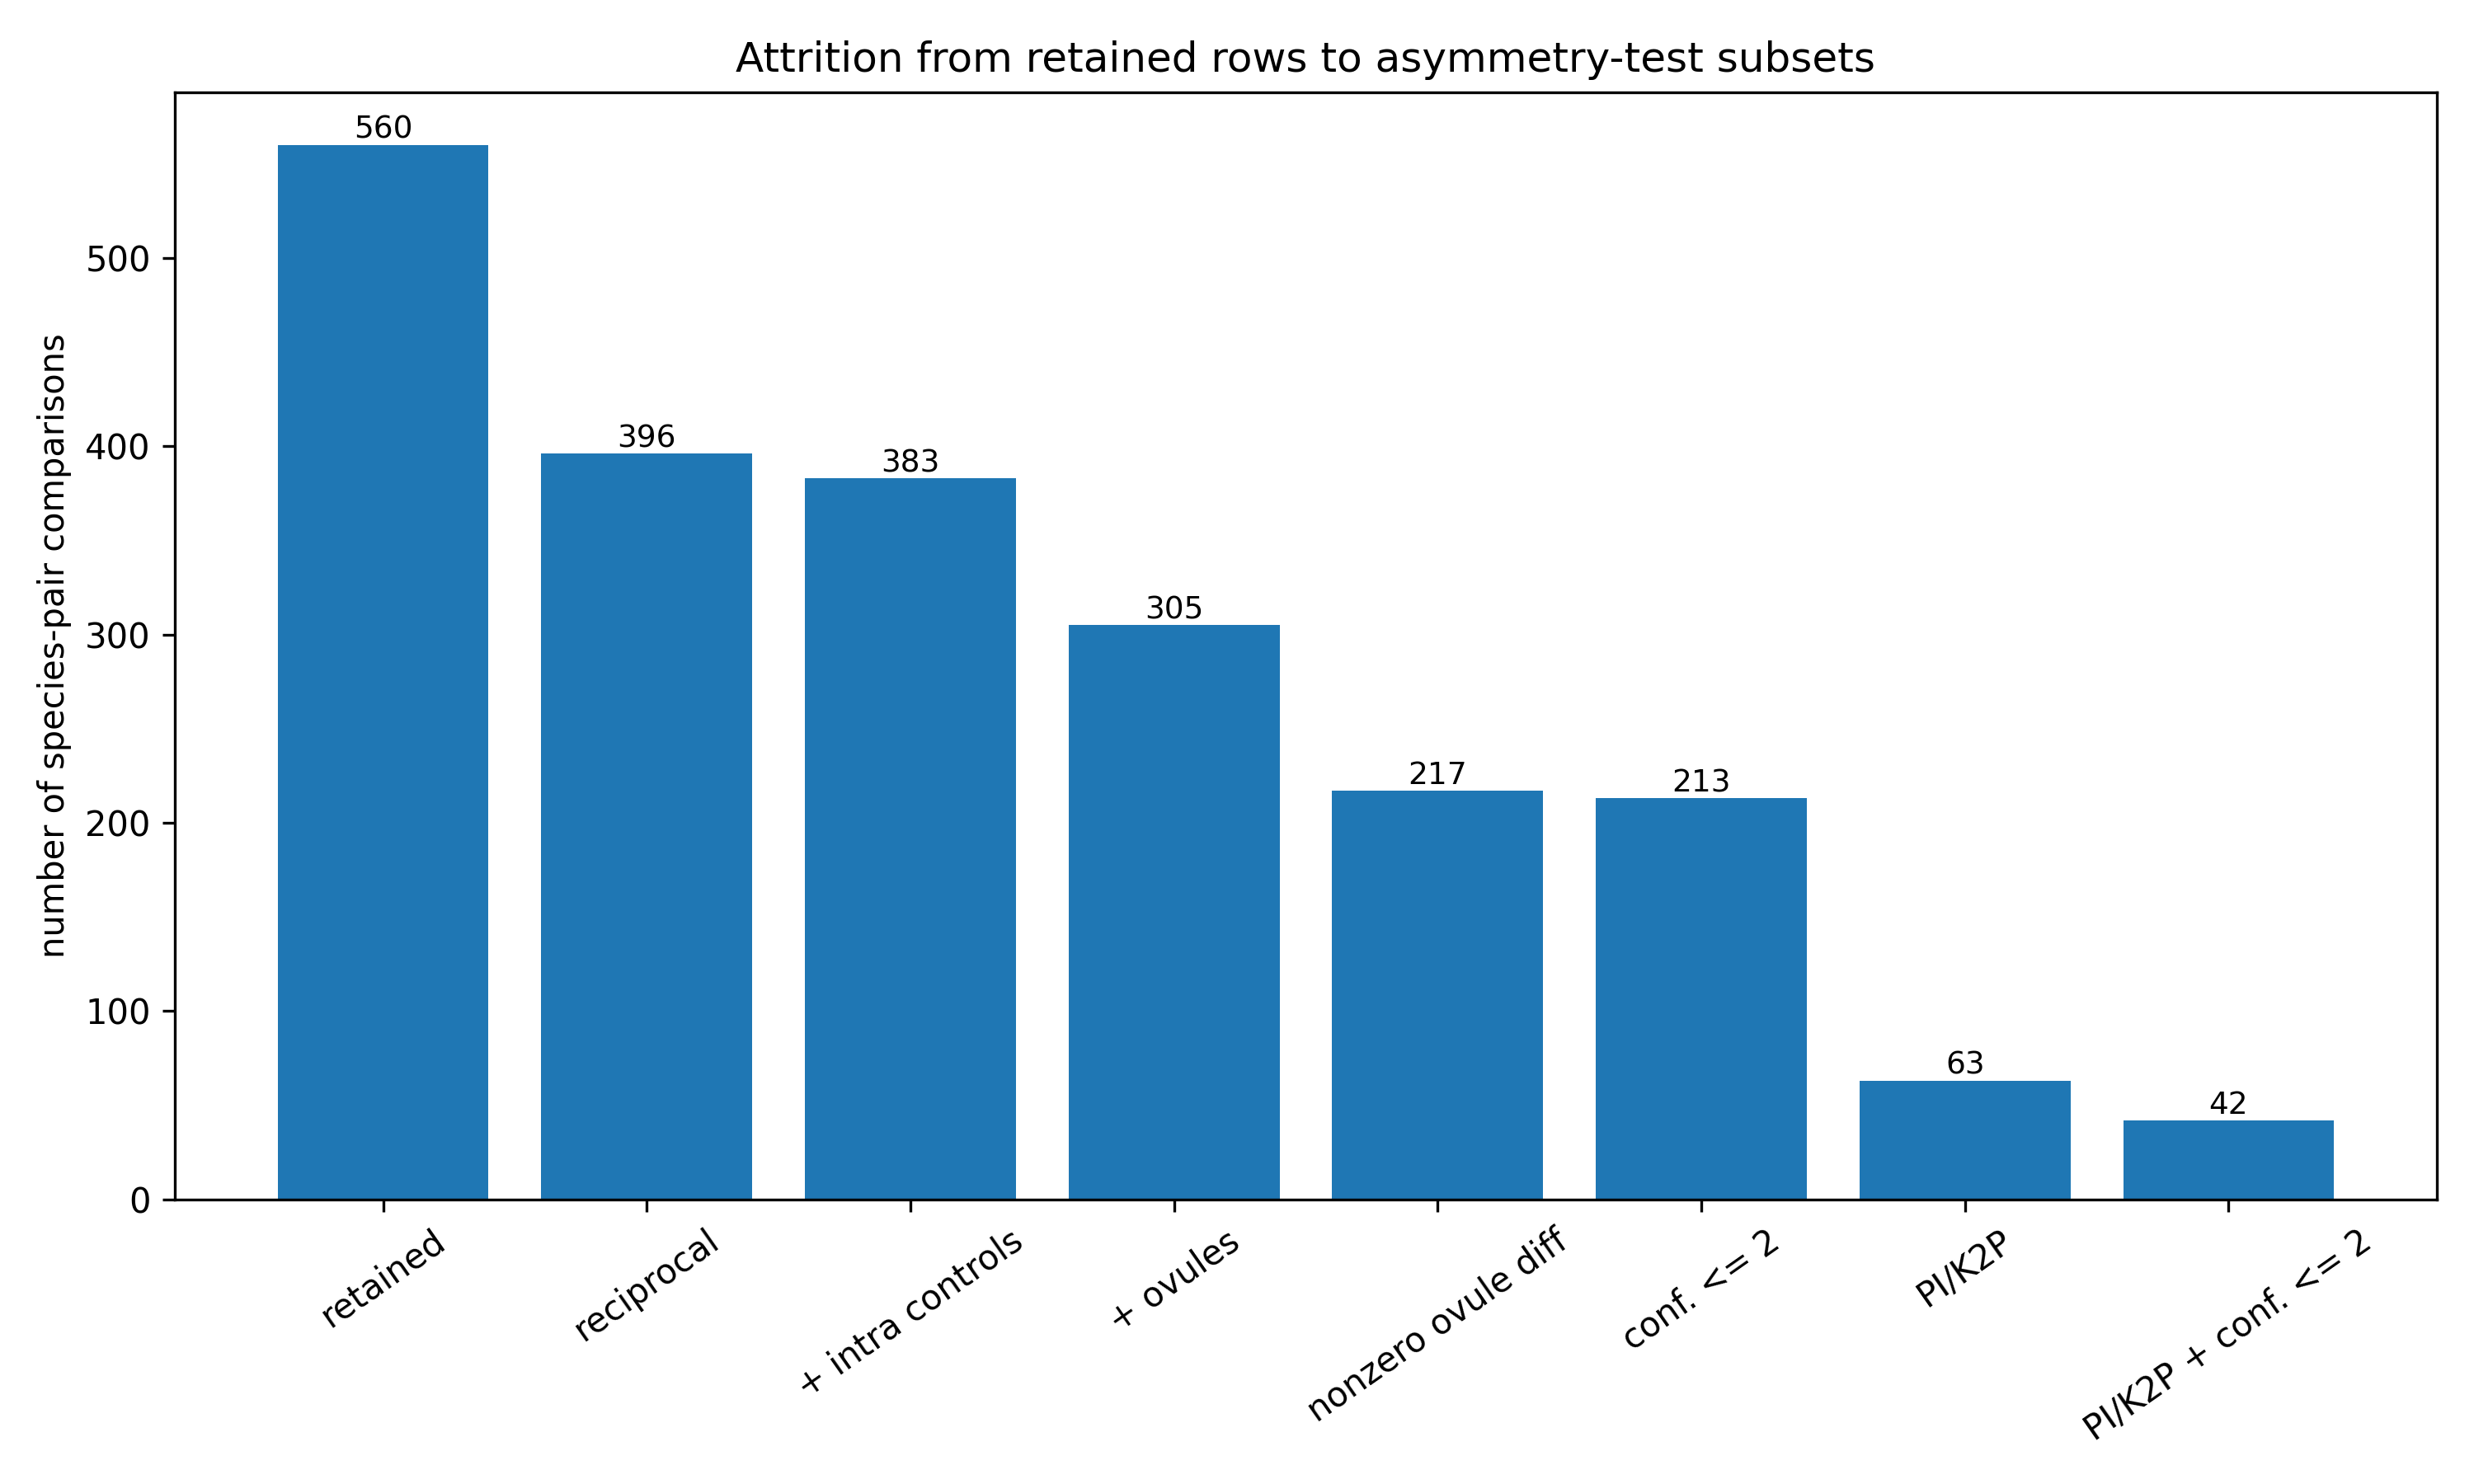
\includegraphics[width=0.95\linewidth]{figures/reciprocal_asymmetry_funnel.png}
\caption{Attrition from all retained pair rows to the reciprocal-cross subsets needed for asymmetric tests. The main asymmetric dataset has 305 species-pair comparisons across 41 families. The strict PI/K2P version has 63 comparisons across 35 families.}
\label{fig:asymmetry-funnel}
\end{figure}

\begin{table}[H]
\centering
\small
\begin{adjustbox}{max width=\linewidth}
\begin{tabular}{>{\raggedright\arraybackslash}p{0.62\linewidth}rr}
\toprule
Dataset condition & Pair comparisons & Families \\
\midrule
Retained pair rows & 560 & 50 \\
Both reciprocal interspecific directions & 396 & 46 \\
Directional RI possible: reciprocal crosses plus both intraspecific controls & 383 & 45 \\
Asymmetry model-ready: directional RI plus both ovule numbers & 305 & 41 \\
Asymmetry model-ready with nonzero ovule difference & 217 & 27 \\
High-confidence ovules only: confidence $\leq 2$ for both species & 213 & 31 \\
Strict PI/K2P asymmetry subset & 63 & 35 \\
Strict PI/K2P plus high-confidence ovules & 42 & 27 \\
\bottomrule
\end{tabular}
\end{adjustbox}
\caption{Data attrition for the reciprocal-cross asymmetric test.}
\label{tab:reciprocal-attrition}
\end{table}

\begin{conclusionbox}
The asymmetric reciprocal-cross test has 305 usable pair comparisons across 41 families. The high-confidence version has 213 comparisons across 31 families. The strict PI/K2P subset is useful, but it is too small to carry the whole paper by itself.
\end{conclusionbox}

\section{Family-level structure}

The data are not evenly spread across families. This is not a nuisance detail. It tells us how to fit the model. Some families carry many reciprocal comparisons and real ovule contrasts. Other families have reciprocal crosses but no ovule contrast. Those latter families can help estimate background asymmetry and measurement noise, but they cannot estimate the ovule-number slope within family.

\begin{figure}[H]
\centering
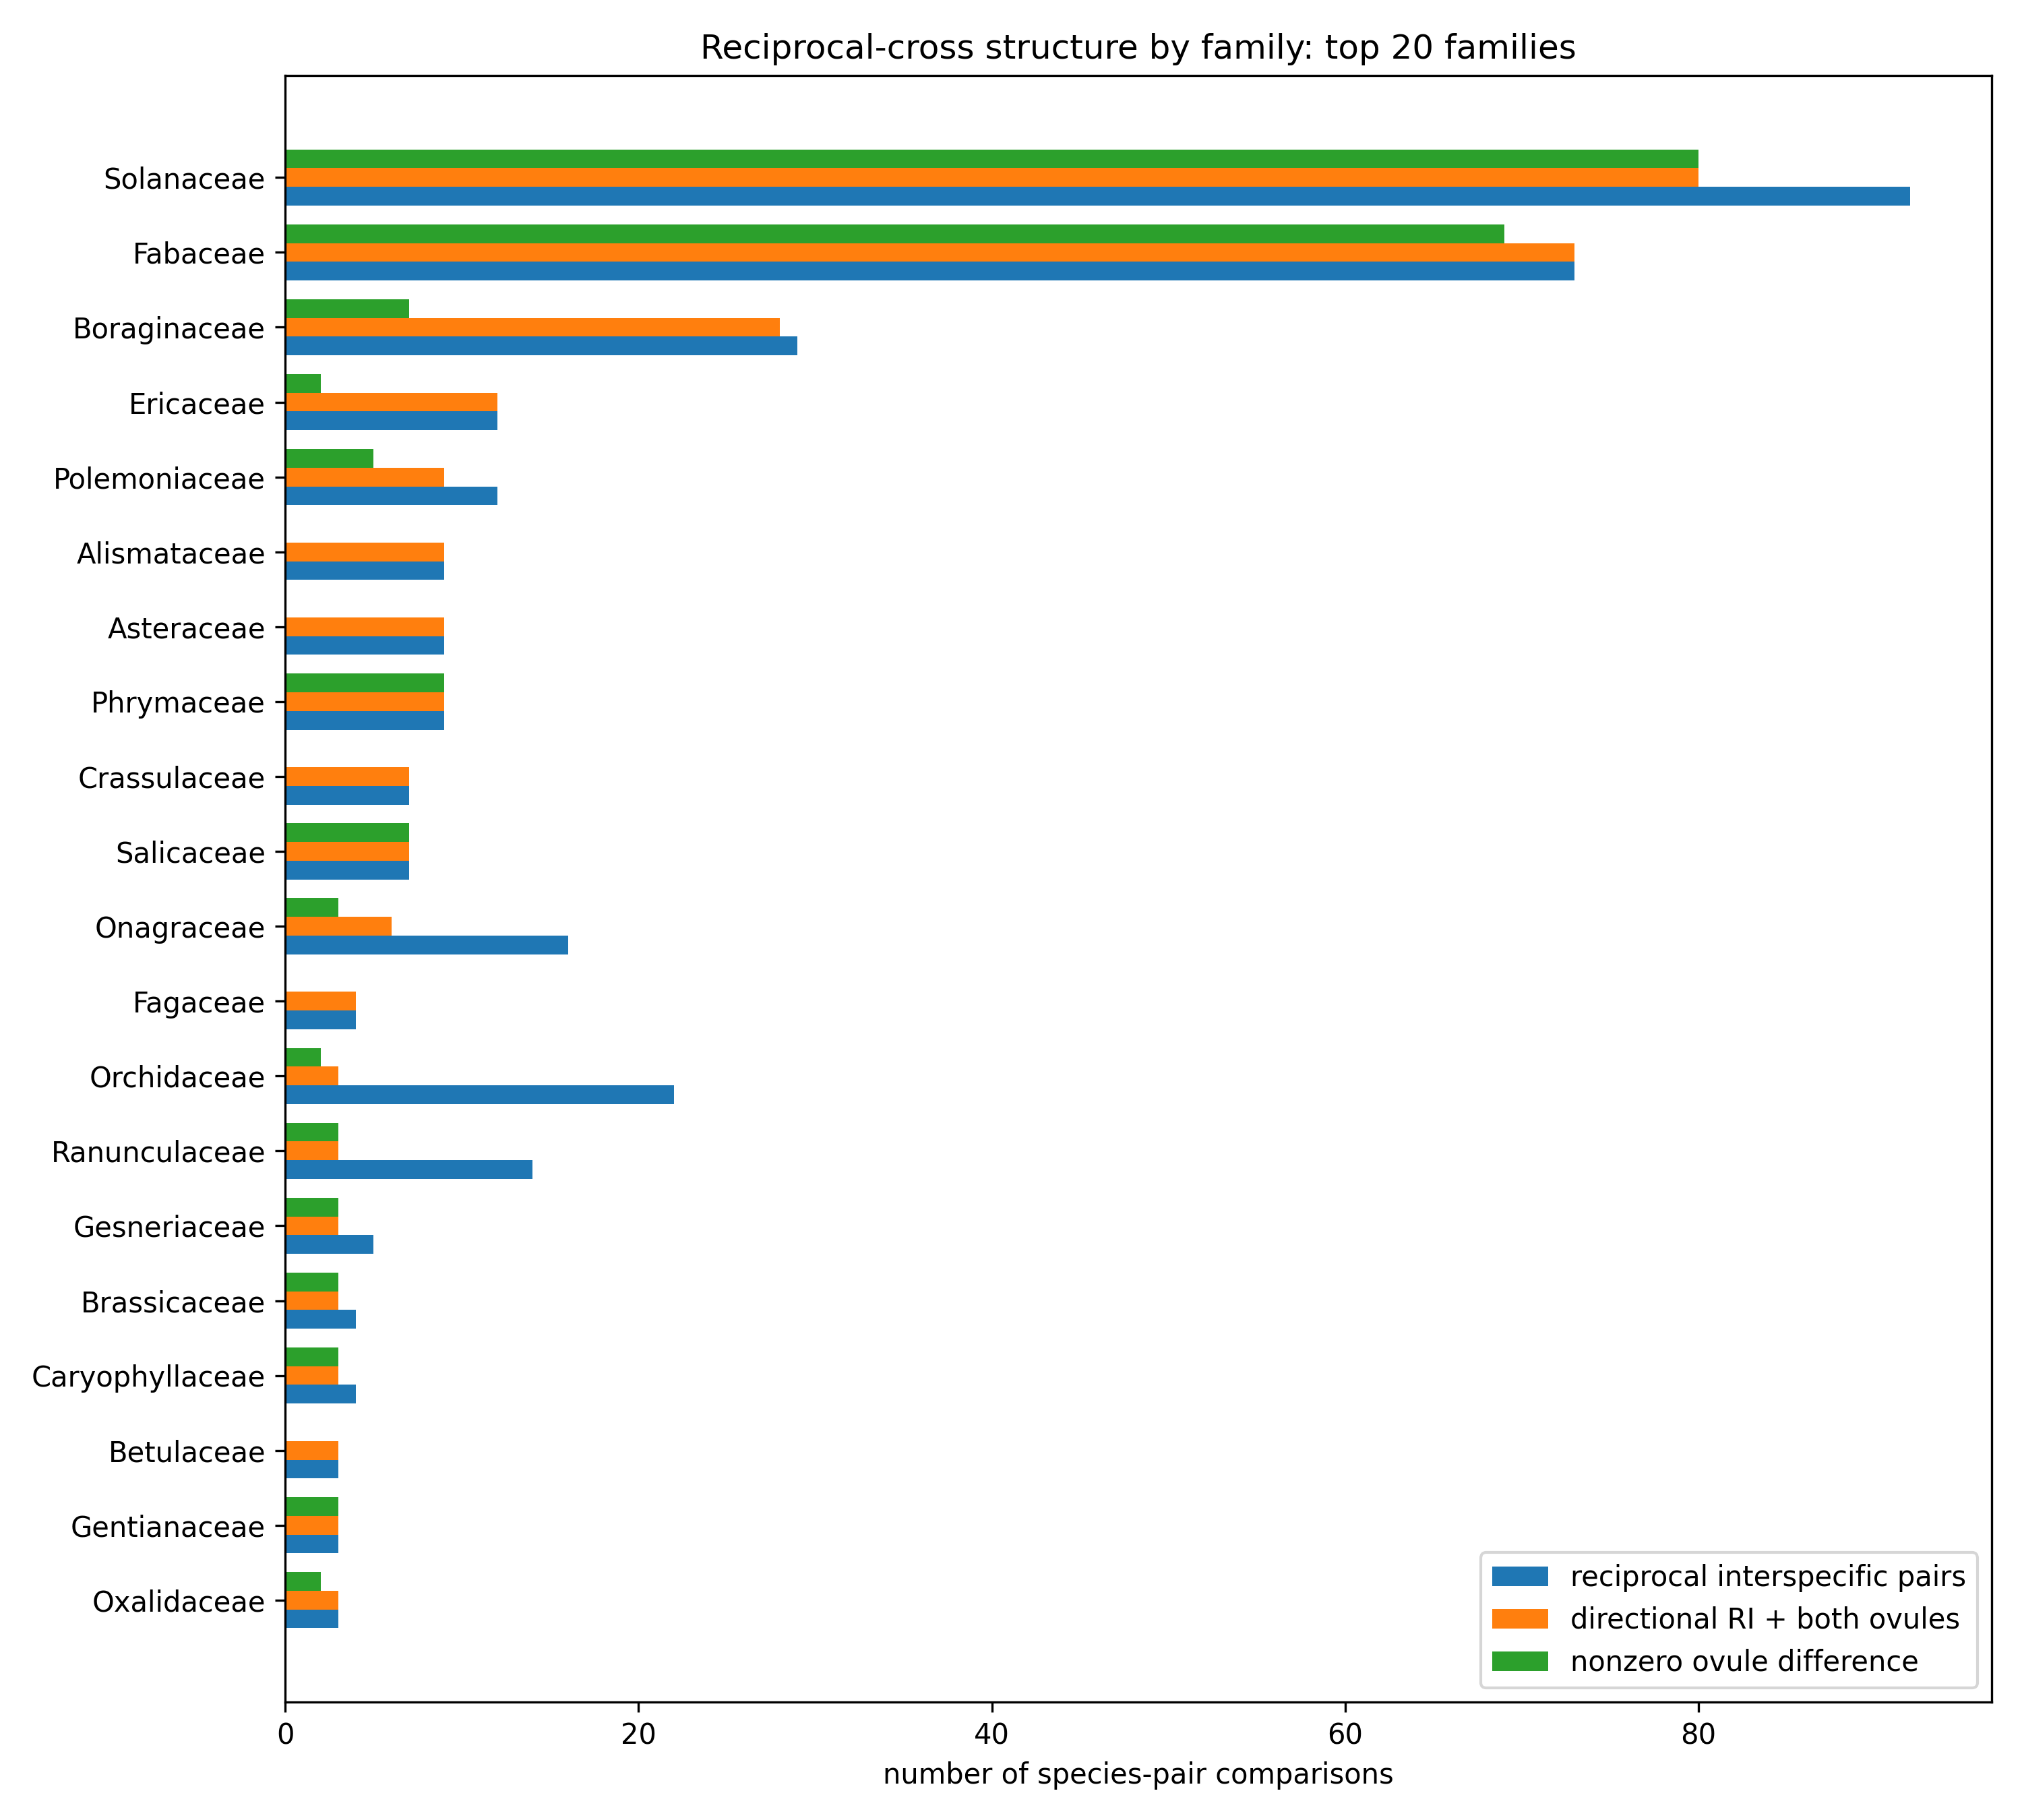
\includegraphics[width=0.98\linewidth]{figures/family_reciprocal_asymmetry_top20.png}
\caption{Family-level reciprocal-cross structure for the 20 largest families. The plotted bars count reciprocal interspecific pairs, pairs with directional RI and both ovule estimates, and pairs with nonzero ovule-number differences.}
\label{fig:family-reciprocal-top20}
\end{figure}

\begin{table}[H]
\centering
\scriptsize
\begin{adjustbox}{max width=\linewidth}
\begin{tabular}{lrrrrrr}
\toprule
Family & Reciprocal & Directional RI & + ovules & Nonzero $\Delta O$ & Conf. $\leq 2$ & PI/K2P \\
\midrule
Solanaceae & 92 & 87 & 80 & 80 & 31 & 7 \\
Fabaceae & 73 & 73 & 73 & 69 & 72 & 8 \\
Boraginaceae & 29 & 28 & 28 & 7 & 28 & 0 \\
Ericaceae & 12 & 12 & 12 & 2 & 1 & 3 \\
Polemoniaceae & 12 & 11 & 9 & 5 & 9 & 2 \\
Alismataceae & 9 & 9 & 9 & 0 & 9 & 1 \\
Asteraceae & 9 & 9 & 9 & 0 & 9 & 2 \\
Phrymaceae & 9 & 9 & 9 & 9 & 1 & 2 \\
Crassulaceae & 7 & 7 & 7 & 0 & 0 & 0 \\
Salicaceae & 7 & 7 & 7 & 7 & 7 & 2 \\
Onagraceae & 16 & 16 & 6 & 3 & 6 & 1 \\
Fagaceae & 4 & 4 & 4 & 0 & 4 & 1 \\
Orchidaceae & 22 & 22 & 3 & 2 & 2 & 3 \\
Ranunculaceae & 14 & 14 & 3 & 3 & 3 & 1 \\
Gesneriaceae & 5 & 5 & 3 & 3 & 0 & 2 \\
Brassicaceae & 4 & 4 & 3 & 3 & 3 & 3 \\
Caryophyllaceae & 4 & 4 & 3 & 3 & 3 & 1 \\
Betulaceae & 3 & 3 & 3 & 0 & 3 & 1 \\
Gentianaceae & 3 & 3 & 3 & 3 & 3 & 1 \\
Oxalidaceae & 3 & 3 & 3 & 2 & 3 & 1 \\
\bottomrule
\end{tabular}
\end{adjustbox}
\caption{Family-level coverage for the asymmetric reciprocal-cross test. ``+ ovules'' means directional RI plus ovule numbers for both species. ``Nonzero $\Delta O$'' means the pair has an ovule-number contrast on the log scale.}
\label{tab:family-coverage}
\end{table}

Solanaceae and Fabaceae supply 153 of the 305 asymmetry-ready comparisons. That gives power, but it also creates leverage. A pooled model could become a Solanaceae--Fabaceae model in disguise. This is why family-level analysis is not optional.

There are 19 families with at least two asymmetry-ready comparisons and at least two distinct signed ovule contrasts. There are 16 families with at least three such comparisons, and eight families with at least five. Under the confidence $\leq 2$ restriction, those numbers fall to 13, 11, and six families.

\begin{table}[H]
\centering
\small
\begin{tabular}{lcc}
\toprule
Minimum family requirement & All numeric ovules & Confidence $\leq 2$ \\
\midrule
At least 2 pairs and at least 2 ovule contrasts & 19 families & 13 families \\
At least 3 pairs and at least 2 ovule contrasts & 16 families & 11 families \\
At least 5 pairs and at least 2 ovule contrasts & 8 families & 6 families \\
\bottomrule
\end{tabular}
\caption{How many families can estimate a within-family ovule-asymmetry slope under different minimum requirements.}
\label{tab:family-slope-capacity}
\end{table}

\begin{conclusionbox}
Do not fit a separate fixed slope for every family. Too many families have few comparisons. The right compromise is partial pooling: estimate a global ovule-asymmetry slope while allowing family slopes to vary around it.
\end{conclusionbox}

\subsection{A partial-pooling model for families}

A practical family model is
\begin{equation}
A^{SC}_{ij}=\alpha+a_{f[ij]}+
\left(\beta+b_{f[ij]}\right)G_{ij}\left[\log_{10}(O_j)-\log_{10}(O_i)\right]
+\gamma_{m[ij]}+u_{s_1[ij]}+u_{s_2[ij]}+\epsilon_{ij}.
\label{eq:family-pooling}
\end{equation}
Here $f[ij]$ is family, $m[ij]$ is measurement type, and $u_{s_1}$ and $u_{s_2}$ are crossed species effects. The random family effects are
\begin{align}
a_f &\sim N(0,\sigma_a^2),\\
b_f &\sim N(0,\sigma_b^2).
\end{align}
This model asks whether the average slope $\beta$ is positive, while allowing families to differ.

If K2P is missing for many reciprocal pairs, fit the model twice. First fit the broader reciprocal model without $G_{ij}$,
\begin{equation}
A^{SC}_{ij}=\alpha+a_{f[ij]}+
\left(\beta+b_{f[ij]}\right)\left[\log_{10}(O_j)-\log_{10}(O_i)\right]
+\gamma_{m[ij]}+u_{s_1[ij]}+u_{s_2[ij]}+\epsilon_{ij}.
\label{eq:family-noG}
\end{equation}
Then fit the strict PI/K2P subset with the interaction term in \eqref{eq:family-pooling}. Agreement in sign across the broad and strict analyses is more informative than any one model alone.

\begin{cautionbox}
Species reuse matters. Fabaceae has many \emph{Leucaena} comparisons, and Boraginaceae is dominated by \emph{Hydrophyllum}. Pairwise observations that share species are correlated. Crossed species effects, phylogenetic covariance, or pairwise comparative methods are needed to avoid overconfident intervals.
\end{cautionbox}

\section{What the current data can and cannot claim}

\subsection{Strengths}

The current datasets have five strong features. First, they contain reciprocal interspecific columns, which are essential for testing a maternal mechanism. Second, they separate cross outcomes from lineage traits, so ovule-number uncertainty can be handled directly. Third, ovule-number confidence categories exist, which makes sensitivity analysis straightforward. Fourth, there is a PI structure and a matching tree for a conservative check. Fifth, the data cover many families, so the result does not have to be presented as a single-clade pattern.

\subsection{Weaknesses}

The main weakness is that the strictest complete-case analysis is much smaller than the broad reciprocal analysis. Requiring reciprocal crosses, both ovule numbers, PI status, and K2P distance leaves 63 asymmetric comparisons. This subset is useful, but it cannot support many interaction terms.

The second weakness is family imbalance. Solanaceae and Fabaceae dominate the model-ready reciprocal data. They should be treated as informative families, not as independent evidence repeated 153 times.

The third weakness is that some families have reciprocal crosses but no ovule contrast. Alismataceae, Asteraceae, Crassulaceae, Fagaceae, and Betulaceae fall into this category in the current audit. These families can estimate background asymmetry but not an ovule-number slope.

The fourth weakness is measurement heterogeneity. Fruit set, seed set, seed number per fruit, and pollen competition do not share the same denominator. A measurement-type effect is mandatory. Stratified sensitivity analyses are also worth doing.

The fifth weakness is that raw denominators are mostly absent. The model is about ovules, pollen, and successful seed production, but the current table contains summary values. That means a beta-binomial or binomial count model is a future target rather than the first analysis.

\begin{conclusionbox}
The current data can test whether reciprocal asymmetry is aligned with signed ovule-number contrast. They cannot yet prove the full causal chain from field pollen load to pollen competition to maternal filtering. That stronger test will need pollen dose, pollen-tube, ovule-exposure, and seed-count denominators.
\end{conclusionbox}

\section{Suggested tools for the first analysis}

Use three linked analyses rather than one large model.

\textbf{Analysis 1: broad reciprocal asymmetry.} Use all 305 asymmetry-ready pairs. Response: $A^{SC}_{ij}$. Predictor: signed log ovule contrast. Include family partial pooling, measure type, ovule confidence, and crossed species effects. This is the power analysis.

\textbf{Analysis 2: high-confidence ovules.} Repeat Analysis 1 with confidence $\leq 2$ for both species. This tests whether the result depends on weak ovule estimates.

\textbf{Analysis 3: strict PI/K2P.} Use the 63 strict comparisons with K2P distance. Fit the theoretical interaction $G_{ij}[\log_{10}(O_j)-\log_{10}(O_i)]$. This is the conservative divergence-scaled test.

In R, the practical route is \texttt{tidyverse} for reshaping, \texttt{ape} for tree checks, \texttt{phylolm} or \texttt{nlme} for simpler phylogenetic models, and \texttt{brms} or \texttt{MCMCglmm} for crossed species effects and phylogenetic covariance. For pairwise comparative structure, \texttt{phylopairs} is worth testing alongside the PI subset. In Python, \texttt{pandas} is enough for the audit, while \texttt{bambi}, \texttt{pymc}, or \texttt{statsmodels} can fit first-pass models.

\begin{cautionbox}
The first model should be boring. If the sign of the ovule-asymmetry effect is not stable in the boring models, a complex phylogenetic Bayesian model will not rescue the claim. Complexity should protect against false certainty, not create the signal.
\end{cautionbox}

\section{Proper statistical analysis of the prediction}

The empirical test should follow the direction of the biology. A broad regression of total RI on ovule number is too blunt because the model is maternal and reciprocal. The proper test asks whether the same species pair fails more strongly in the direction where the maternal parent has fewer ovules.

\subsection{Keep the sign convention fixed}

For species pair $(1,2)$, define
\begin{equation}
A^{SC}_{12}=R^{SC}_{1\leftarrow 2}-R^{SC}_{2\leftarrow 1},
\label{eq:analysis-A-SC}
\end{equation}
and
\begin{equation}
\Delta\log O_{12}=\log(O_2)-\log(O_1).
\label{eq:analysis-dlogO}
\end{equation}
This convention is useful because it makes the prediction positive. If species 1 has fewer ovules than species 2, then $O_1<O_2$ and $\Delta\log O_{12}>0$. The model says species 1 should then have the stricter maternal filter. Therefore $R^{SC}_{1\leftarrow 2}>R^{SC}_{2\leftarrow 1}$ and $A^{SC}_{12}>0$.

The first test is therefore
\begin{equation}
A^{SC}_{12}=\beta_0+\beta_O\Delta\log O_{12}+\epsilon_{12},
\label{eq:first-plain-analysis}
\end{equation}
with
\begin{equation}
\boxed{\beta_O>0.}
\end{equation}

\begin{conclusionbox}
The sign convention is not cosmetic. It is a logic check. A positive coefficient means that the fewer-ovule maternal direction has the stronger prezygotic barrier.
\end{conclusionbox}

\subsection{The main model should be paired and family-aware}

The broad model in \eqref{eq:first-plain-analysis} is only a diagnostic. The main model should recognise four features of the data: families differ, species are reused across pairwise comparisons, measurement type differs, and ovule-number confidence varies.

A practical hierarchical model is
\begin{equation}
A^{SC}_{ij}\sim t_{\nu}(\mu_{ij},\sigma),
\label{eq:t-main-analysis}
\end{equation}
where
\begin{align}
\mu_{ij}={}&\beta_0+
\beta_O\Delta\log O_{ij}
+\gamma_{m[ij]}
+\eta_q q_{ij}
+a_{f[ij]}
+b_{f[ij]}\Delta\log O_{ij}
+u_i-u_j .
\label{eq:main-analysis-mu}
\end{align}
Here $m[ij]$ is measurement type, $q_{ij}$ is an ovule-confidence or ovule-provenance term, $f[ij]$ is family, and $u_i-u_j$ represents repeated species effects. The family effects are partially pooled:
\begin{align}
a_f&\sim N(0,\sigma_a^2),\\
b_f&\sim N(0,\sigma_b^2).
\end{align}
The family-specific ovule slopes are
\begin{equation}
\beta_{O,f}=\beta_O+b_f.
\end{equation}
The important questions are then
\begin{align}
\Pr(\beta_O>0\mid \mathrm{data}),
\end{align}
and, for each family,
\begin{align}
\Pr(\beta_{O,f}>0\mid \mathrm{data}).
\end{align}

\begin{cautionbox}
The family analysis should use partial pooling. Separate fixed-effect slopes for every family are descriptive, not the main inference, because many families have too few pairs or too little ovule contrast.
\end{cautionbox}

\subsection{Use the divergence-scaled model as a strict sensitivity analysis}

The theory predicts that asymmetry needs both a maternal-filter contrast and mismatch. If K2P distance is available, fit
\begin{equation}
A^{SC}_{ij}=\beta_0+\beta_O\Delta\log O_{ij}+\beta_GG_{ij}+\beta_{GO}G_{ij}\Delta\log O_{ij}+\epsilon_{ij}.
\label{eq:strict-G-analysis}
\end{equation}
The most mechanistic prediction is
\begin{equation}
\boxed{\beta_{GO}>0.}
\end{equation}
This subset is smaller than the full reciprocal dataset, so it should not replace the broad reciprocal test. Instead it asks whether the directional ovule effect strengthens with genetic distance.

\subsection{The long-form paired model is the same test}

The same analysis can be written with two rows per species pair:
\begin{equation}
R^{SC}_{i\leftarrow j}=\alpha_{ij}+\beta_M[-\log(O_i)]+\varepsilon_{i\leftarrow j}.
\label{eq:long-pair-analysis}
\end{equation}
The pair effect $\alpha_{ij}$ absorbs everything symmetric about the pair: genetic distance, general compatibility, study effects, and pair-level fecundity. With two reciprocal directions, this model is algebraically equivalent to a paired difference model using $A^{SC}_{ij}$ and $\Delta\log O_{ij}$. It is a useful check because it makes the maternal nature of the prediction explicit.

\subsection{Raw counts would be better than summary RI}

If the original studies provide denominators, the preferred model should use counts rather than RI summaries. For directed cross $i\leftarrow j$, write
\begin{equation}
Y_{i\leftarrow j}\sim \mathrm{BetaBinomial}(N_{i\leftarrow j},p_{i\leftarrow j},\phi),
\label{eq:raw-count-analysis}
\end{equation}
where $N_{i\leftarrow j}$ is the relevant denominator and $Y_{i\leftarrow j}$ is the number of successes. The denominator must match the measurement: pollinations, flowers, fruits, ovules, or seeds. A directed count model is
\begin{equation}
\logit(p_{i\leftarrow j})=\alpha_{ij}
+\beta_M[-\log(O_i)]
+\beta_{GM}G_{ij}[-\log(O_i)]
+\gamma_{m[ij]}+u_i^{(M)}+u_j^{(P)}.
\label{eq:raw-count-regression}
\end{equation}
This would be the strongest version of the analysis because it keeps denominator information instead of compressing it into a single index.

\subsection{Separate the ovule model from unilateral incompatibility}

Mating system is useful but not enough. Selfing, mixed mating, and outcrossing do not map perfectly onto self-incompatibility status. If SI status can be coded, the discriminating model should be
\begin{equation}
A^{SC}_{ij}=\beta_0+\beta_O\Delta\log O_{ij}
+\beta_{GO}G_{ij}\Delta\log O_{ij}
+\beta_{SI}\Delta SI_{ij}
+\beta_t\bar{t}_{ij}\Delta\log O_{ij}
+\gamma_{m[ij]}+\epsilon_{ij}.
\label{eq:SI-discriminating-analysis}
\end{equation}
The ovule-gated model predicts positive $\beta_O$ or $\beta_{GO}$. The unilateral-incompatibility model predicts that $\beta_{SI}$ should carry the direction.

\begin{cautionbox}
Do not treat the Table 2 mating-system category as SI status. It is a useful modifier of pollen-donor diversity, but SI requires a separate coding if we want to distinguish mechanisms.
\end{cautionbox}

\subsection{Phylogenetic and pairwise non-independence}

Species-pair data reuse species. They also reuse clades. If $C$ is the species-level phylogenetic covariance matrix and $L$ is a contrast matrix with $+1$ for species 1 and $-1$ for species 2, then a pairwise phylogenetic covariance can be written as
\begin{equation}
V_{\mathrm{pair}}=LCL^{\top}.
\label{eq:pairwise-phylo-covariance}
\end{equation}
A phylogenetic version of the asymmetry model is then
\begin{equation}
A\sim N(\mu,\sigma^2V_{\mathrm{pair}}+\sigma_e^2I).
\label{eq:phylo-analysis}
\end{equation}
This is the right comparative structure for pairwise traits. The PI/K2P subset remains useful as a conservative check, but the pairwise covariance model is the better target when the tree is cleaned.

\subsection{Diagnostics that should be reported}

The paper should report seven diagnostics.

\begin{enumerate}
\item A raw quadrant plot of $A^{SC}_{ij}$ against $\Delta\log O_{ij}$.
\item The broad reciprocal slope, the high-confidence ovule slope, and the strict PI/K2P interaction slope.
\item Family-specific descriptive slopes, with the global conclusion based on partial pooling rather than fixed slopes for every family.
\item Leave-one-family-out fits, especially removing Solanaceae and Fabaceae.
\item A within-family permutation test that shuffles ovule numbers among species while keeping the cross network fixed.
\item A negative-control summary for pairs with zero or nearly zero ovule contrast.
\item A model including SI status once those data are curated.
\end{enumerate}

\subsection{Executable first-pass analysis}

I wrote a Python script that builds the analysis table and runs the first diagnostic models. The script uses Table 1 for cross outcomes, Table 2 for ovule number, confidence, life history, and mating system, Table 2b for exact species-level ovule-fill auditing, and the K2P file for the strict divergence-scaled subset.

The command is
\begin{verbatim}
python scripts/ovule_asymmetry_analysis.py \
  --input-dir . \
  --output-dir ovule_prediction_analysis_update \
  --n-permutations 999
\end{verbatim}
The main output files are \verb|data/reciprocal_pair_level_SC.csv| and \verb|data/directional_pair_level_SC.csv|. The first has one row per species pair. The second has two rows per pair, one for each maternal direction.

\begin{figure}[H]
\centering
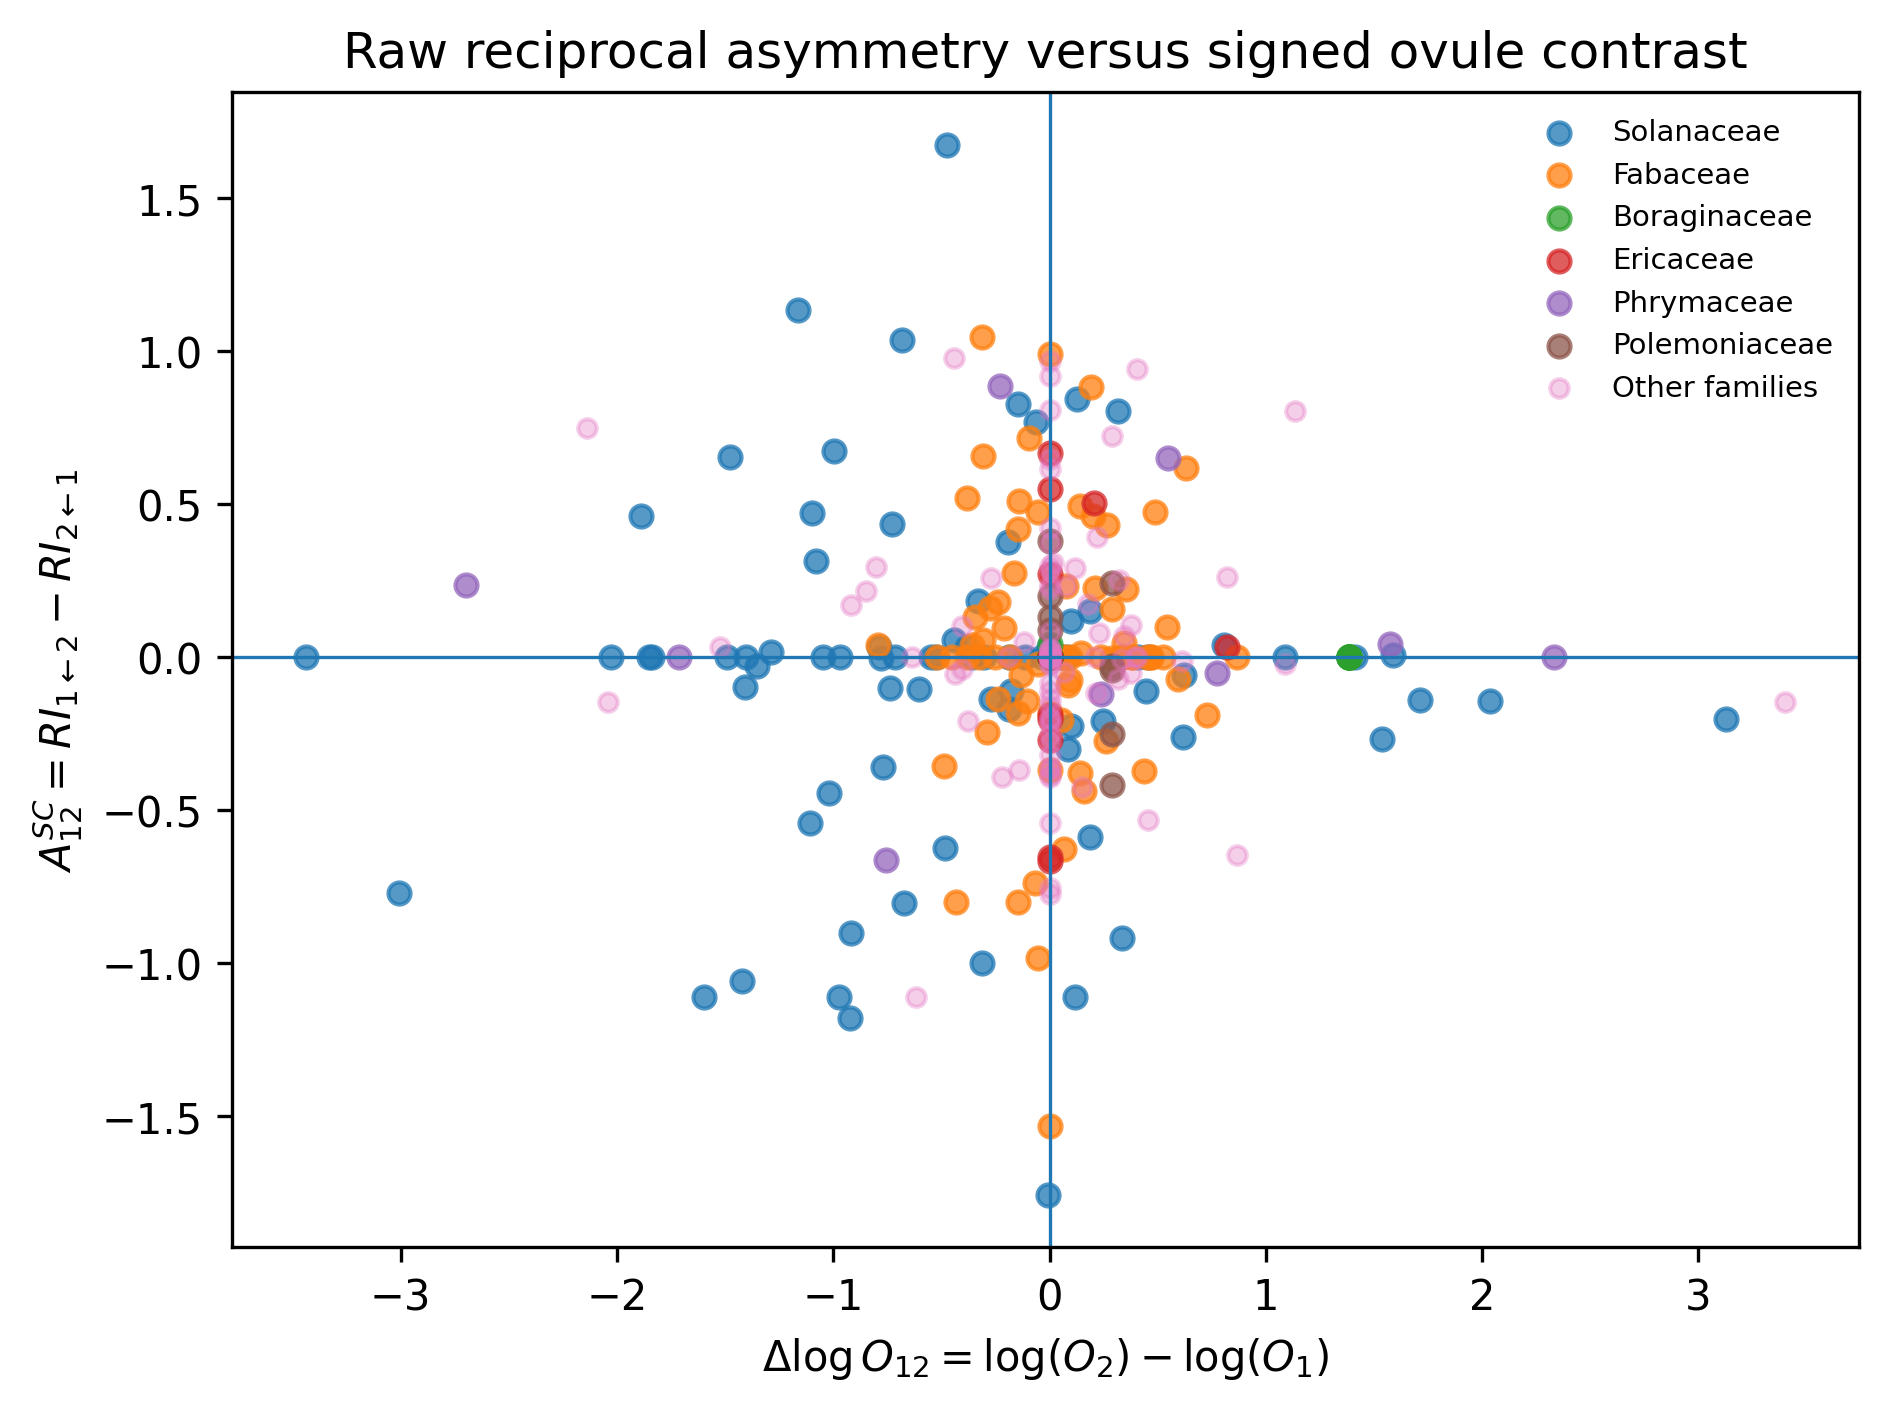
\includegraphics[width=0.90\linewidth]{asymmetry_vs_signed_ovule_contrast.png}
\caption{Raw reciprocal asymmetry against signed ovule contrast. The predicted signal is a positive association: points should tend to fall in the upper-right and lower-left quadrants. This figure is a diagnostic, not the final model.}
\label{fig:raw-asymmetry-analysis-diagnostic}
\end{figure}

\begin{table}[H]
\centering
\small
\begin{adjustbox}{max width=\linewidth}
\begin{tabular}{lrrlll}
\toprule
Subset & $n$ & Sign test $n$ & Agreement & Pearson $r$ & $p_+$ \\
\midrule
All asymmetry-ready & 305 & 163 & 0.479 & 0.021 & 0.734 \\
High-confidence ovules & 213 & 112 & 0.446 & -0.127 & 0.890 \\
Strict PI/K2P & 63 & 36 & 0.472 & -0.099 & 0.691 \\
\bottomrule
\end{tabular}
\end{adjustbox}
\caption{Raw sign and correlation checks. The sign test excludes exact zeros in both the response and the ovule contrast. A value above 0.5 would indicate more agreement with the predicted quadrant structure than expected by chance.}
\label{tab:sign-checks}
\end{table}


\begin{table}[H]
\centering
\small
\begin{adjustbox}{max width=\linewidth}
\begin{tabular}{lrllll}
\toprule
Analysis & $n$ & Target & $\hat{\beta}$ & SE & $p_{+}$ \\
\midrule
Broad reciprocal, measure adjusted & 305 & $\Delta\log O$ & 0.019 & 0.032 & 0.269 \\
Broad reciprocal, family + measure fixed effects & 305 & $\Delta\log O$ & 0.010 & 0.029 & 0.364 \\
High-confidence ovules, family + measure & 213 & $\Delta\log O$ & -0.053 & 0.055 & 0.830 \\
Strict PI/K2P divergence interaction & 63 & $G\Delta\log O$ & -2.309 & 4.639 & 0.691 \\
Directional pair fixed-effect equivalent & 217 & $\Delta\log O$ & 0.012 & 0.031 & 0.355 \\
\bottomrule
\end{tabular}
\end{adjustbox}
\caption{First-pass executable checks of the reciprocal asymmetry prediction. The one-sided value $p_{+}$ tests the directional prediction that the target coefficient is positive. These checks are diagnostics, not the final phylogenetic mixed model.}
\label{tab:first-pass-analysis-checks}
\end{table}


The first executable checks do not yet show a stable positive signal. The broad measure-adjusted slope is positive but small; the family-adjusted slope is also small; the high-confidence subset is negative; and the strict PI/K2P interaction is negative with a large standard error. The within-family permutation test gives a one-sided positive-tail value of about $0.39$ for the family-and-measure residualised slope. These results should be treated as a warning, not a failure of the project. They say that the current summary data do not give an immediate pooled signal. The next test should ask whether the prediction appears after better mechanism coding, especially SI status, raw denominators, pollen-competition stage, and phylogenetic covariance.

\begin{conclusionbox}
The current best test is clear even if the first-pass signal is weak: use reciprocal Sobel--Chen asymmetry as the response, signed ovule contrast as the directional predictor, family partial pooling, repeated-species or phylogenetic covariance, measurement-type effects, ovule-confidence sensitivity, and SI status as the key alternative mechanism.
\end{conclusionbox}


\section{Immediate data-cleaning checklist}

Before fitting the models, make these changes.

\begin{enumerate}
\item Add an explicit Boolean \texttt{is\_PI} column to Table 1. Keep \texttt{PI\_name} as the tree label.
\item Confirm the reciprocal direction of \texttt{interspecific\_value\_sp2\_sp1} against the source spreadsheet.
\item Collapse duplicate genetic-distance rows and keep one K2P value per unordered species pair.
\item Resolve the duplicated \texttt{Corymbia} tree tip before constructing phylogenetic covariance matrices.
\item Recompute directional RI using the exact Sobel--Chen formula in \eqref{eq:SCdata1simple}--\eqref{eq:SCdata2simple}.
\item Mark whether each pair has a nonzero signed ovule contrast. Families with no contrast should not be used to estimate within-family ovule slopes.
\item Keep measurement type in every model and run stratified checks for seed set and fruit set.
\end{enumerate}

\begin{conclusionbox}
The next file we should build is a single analysis table with one row per reciprocal pair and the following fields: family, genus, species 1, species 2, measure, exact directional RI in both directions, exact asymmetry, both ovule numbers, both ovule confidence scores, signed log ovule contrast, mating-system contrast, life-history contrast, K2P distance, PI flag, and tree labels.
\end{conclusionbox}

\section{Missing data}

\subsection{Missing pollen-load data}

Direct pollen-load data are unavailable for the present analysis. This is a limitation, but it does not stop the model. Treat pollen load as a latent quantity.

The simplest approach is sensitivity analysis:
\begin{equation}
\psi\in\{0.001,0.003,0.01,0.02,0.05,0.10\},
\end{equation}
and
\begin{equation}
\alpha\in\{0.25,0.50,0.75,1.00,1.25\}.
\end{equation}
For each combination, compute
\begin{equation}
K_i=\psi cO_i^{\alpha-1}.
\end{equation}
Then ask whether the same qualitative result appears across a broad region of the grid.

A Bayesian latent-variable model is
\begin{equation}
\log K_i=\mu_K+(\alpha-1)\log O_i+\eta_t\logit(t_i)+u_i+\epsilon_i,
\label{eq:latentK}
\end{equation}
where $u_i$ is a phylogenetic effect and $\epsilon_i$ is lineage-specific noise. The term $\eta_t\logit(t_i)$ allows outcrossing rate to modify effective pollen competition.

\begin{conclusionbox}
The missing pollen-load data become a calibration problem. The model is more credible if the sign of the prediction depends on $\alpha<1$, not on one tuned value of $\psi$.
\end{conclusionbox}

\subsection{Missing reciprocal crosses}

Reciprocal crosses are central because the strongest prediction is directional. If only one cross direction is available, the data can test whether few-ovule lineages have stronger RI on average. They cannot test the maternal-filter prediction cleanly.

\subsection{Missing mating-system data}

If outcrossing rate is missing, code broad categories with uncertainty:
\begin{equation}
t_i\in\{\hbox{selfing},\hbox{mixed},\hbox{outcrossing}\}.
\end{equation}
Then run the analysis under alternative codings. For example, assign approximate values
\begin{equation}
t_i=0.05,\;0.50,\;0.95
\end{equation}
for selfing, mixed, and outcrossing. Then repeat with wider values. The goal is to test whether the ovule signal depends on implausible mating-system assignments.

\subsection{Worst-to-best data scenarios}

\begin{center}
\begin{tabular}{>{\raggedright\arraybackslash}p{0.20\linewidth} >{\raggedright\arraybackslash}p{0.28\linewidth} >{\raggedright\arraybackslash}p{0.25\linewidth} >{\raggedright\arraybackslash}p{0.17\linewidth}}
\toprule
Scenario & Available data & Claim allowed & Main risk \\
\midrule
Worst publishable & Ovule number, summary RI, rough phylogeny & Theory plus suggestive comparative pattern & Cannot estimate $K$ or direction well \\
Minimal directional & Ovule number, genetic distance, some reciprocal RI & Test sign of asymmetry with ovule contrast & Pollen load and mating system inferred \\
Solid comparative & Raw cross counts, ovule denominators, reciprocals, postzygotic data, phylogeny & Test prezygotic-postzygotic decoupling & $K$ still partly latent \\
Strong mechanistic & Adds pollen tubes, pollen production, mating system, SI status & Locate barrier and separate UI & Field pollen load still limited \\
Best empirical & Adds natural pollen load, donor diversity, timing, manipulative pollen-dose experiments & Test the causal chain directly & Hardest to collect \\
\bottomrule
\end{tabular}
\end{center}

\section{Simulation protocol}

The simulation should answer two questions. First, does the mathematical mechanism behave as expected? Second, what data structures can recover the mechanism?

\subsection{Layer 1: ecological competition without RI}

Simulate lineages with ovule number $O_i$. For each lineage, simulate effective pollen load using
\begin{equation}
P_{if}\sim \mathrm{NegBinomial}(\mu_i,\theta_P),
\end{equation}
where
\begin{equation}
\mu_i=\psi cO_i^\alpha.
\end{equation}
Compute
\begin{equation}
K_{if}=P_{if}/O_i
\end{equation}
and
\begin{equation}
S_z(K_{if})
\end{equation}
using \eqref{eq:Sz}.

Record mean $K$, $\Omega$, and $S_z$ for each lineage. This layer tests only the competition engine.

\subsection{Layer 2: evolving maternal filters}

Let filter strictness evolve toward
\begin{equation}
F_i^*=F_{\max}\frac{K_i}{K_i+K_{50}},
\label{eq:Fsimulation}
\end{equation}
where $F_{\max}$ is the maximum filter and $K_{50}$ is the value of $K$ at which the filter reaches half of $F_{\max}$.

This simulation function is simpler than the fitness model above. It keeps the key property:
\begin{equation}
\frac{dF^*}{dK}>0.
\end{equation}

Simulate mismatch as
\begin{equation}
D_{ij}=\delta_DG_{ij}+D^{\mathrm{arch}}_{ij},
\end{equation}
where $D^{\mathrm{arch}}_{ij}$ depends on genetic architecture.

\subsection{Layer 3: genetic architectures}

Use three architectures.

\textbf{Independent architecture.} Pollen-performance loci and compatibility loci are unlinked. Selection changes pollen performance, but RI evolves slowly unless mismatch also accumulates.

\textbf{Linked architecture.} Pollen-performance loci are linked to compatibility loci. Hitchhiking strength can be approximated by
\begin{equation}
H(r,s)=\frac{s}{s+r},
\end{equation}
where $s$ is the selected effect and $r$ is recombination. Low recombination strengthens passenger RI.

\textbf{Pleiotropic architecture.} The same allele affects pollen performance and compatibility. Let the association between performance effects and mismatch effects be $\rho_{a,d}$. Passenger RI should evolve fastest when $\rho_{a,d}$ is high.

\begin{conclusionbox}
The expected order is pleiotropy $>$ linkage $>$ independence for speed and strength of passenger RI.
\end{conclusionbox}

\subsection{Layer 4: phylogenetic embedding}

Simulate trees with different sizes:
\begin{equation}
n\in\{30,60,120,240\}.
\end{equation}
Simulate ovule number under three models:
\begin{enumerate}
\item Brownian motion on $\log O$;
\item an Ornstein--Uhlenbeck model on $\log O$;
\item a discrete transition model between few-ovule and many-ovule regimes.
\end{enumerate}

The third model matters most for the comparative question because it counts independent transitions.

\subsection{Layer 5: crossing data}

For each pair, compute
\begin{equation}
R_{i\leftarrow j}=\tanh\left(\frac{F_iD_{ij}}{2}\right),
\end{equation}
\begin{equation}
R_{j\leftarrow i}=\tanh\left(\frac{F_jD_{ij}}{2}\right),
\end{equation}
and
\begin{equation}
A_{ij}=R_{i\leftarrow j}-R_{j\leftarrow i}.
\end{equation}

Simulate observed seed counts:
\begin{equation}
Y_{i\leftarrow j}\sim \mathrm{BetaBinomial}(N_{i\leftarrow j},1-R_{i\leftarrow j},\theta).
\end{equation}

Simulate postzygotic RI from \eqref{eq:BDM} and \eqref{eq:Rpost}.

\subsection{Layer 6: damage the data}

Create data structures from best to worst:
\begin{enumerate}
\item all reciprocal crosses, raw counts, pollen load, SI status, mating system;
\item reciprocal crosses and raw counts, but no pollen load;
\item reciprocal crosses for a sparse set of pairs;
\item one-direction crosses only;
\item summary proportions only;
\item family-level states only.
\end{enumerate}
For each structure, fit \eqref{eq:empiricalA} or \eqref{eq:discrim}. Record bias, power, false-positive rate, and sign recovery.

\subsection{Core simulation outputs}

Record
\begin{equation}
K_i,\quad K_{\mathrm{sex},i},\quad \Omega_i,\quad S_z(K_i),\quad F_i,\quad D_{ij},\quad R_{i\leftarrow j},\quad A_{ij},\quad \Rpost_{ij}.
\end{equation}
Also record genomic summaries:
\begin{align*}
&\hbox{number of sweeps},\\
&\hbox{mean sweep strength},\\
&\hbox{fraction of sweeps affecting compatibility},\\
&\hbox{fraction of hitchhiked compatibility alleles}.
\end{align*}

\begin{conclusionbox}
The simulation should be judged by recovery, not by appearance. The main recovery target is a positive coefficient for $G_{ij}(\log O_j-\log O_i)$ after accounting for SI status and mating system.
\end{conclusionbox}

\section{Collaborator checklist}

Before analysing the real data, answer these questions.

\begin{enumerate}
\item Do we have reciprocal crosses for the pairs that matter most? The current answer is yes for 396 retained pairs, and 305 also have both ovule estimates.
\item Which families estimate the ovule slope rather than only background asymmetry? The current answer is about 19 families under a lenient rule and eight under a five-pair rule.
\item Are the few-ovule taxa also mostly self-incompatible?
\item Are the many-ovule taxa also mostly self-compatible?
\item Do we have raw counts or only summary RI values?
\item Do we know whether the barrier acts at stigma, style, ovary, ovule, seed set, or F1 fertility?
\item Do we know mating system well enough to separate selfers, mixed-maters, and outcrossers?
\item Are few-ovule states replicated across the phylogeny, or concentrated in one clade?
\item Does asymmetry occur at intermediate divergence, where the model says it should be most visible?
\item Does the sign of the exact Sobel--Chen asymmetry agree with the sign of the simpler diagnostic ratio asymmetry?
\end{enumerate}

\begin{conclusionbox}
The strongest test is not a correlation between ovule number and RI. The strongest test is directional: reciprocal asymmetry should follow maternal competition state, after controlling for divergence, SI status, mating system, and phylogeny.
\end{conclusionbox}

\section{Summary of the model}

The model can be written as one causal chain:
\begin{equation}
O_i \rightarrow K_i=\frac{P_{\mathrm{eff},i}}{O_i} \rightarrow S_z(K_i) \rightarrow
F_i^*(K_i) \rightarrow R_{i\leftarrow j}.
\end{equation}
Under sublinear pollen-load scaling,
\begin{equation}
P_{\mathrm{eff},i}=\psi cO_i^\alpha,\quad \alpha<1,
\end{equation}
so
\begin{equation}
K_i=\psi cO_i^{\alpha-1}.
\end{equation}
Few-ovule lineages then have higher $K$. Higher $K$ strengthens pollen competition and makes maternal filtering less costly. When pollen-pistil mismatch exists between lineages, stricter maternal filtering creates directional prezygotic RI.

The central empirical approximation is
\begin{equation}
A_{ij}\approx \beta_1G_{ij}(\log O_j-\log O_i),
\quad \beta_1>0.
\end{equation}
This prediction should be strongest in outcrossing or mixed-mating lineages with genetically diverse pollen loads. It should weaken in predominant selfers.

\begin{conclusionbox}
The claim is narrow enough to test. Reproductive isolation is not treated as an inevitable clock. Prezygotic RI can be regenerated when reproductive ecology places lineages in a high pollen-competition state.
\end{conclusionbox}

\newpage
\addcontentsline{toc}{section}{References}

\begin{thebibliography}{99}

\bibitem[Anderson et~al.(2025)]{Anderson2025}
Anderson, S. A. S., and colleagues. 2025. The comparative analysis of lineage-pair traits. \emph{Systematic Biology}. doi:10.1093/sysbio/syaf061.

\bibitem[Lankinen and Karlsson Green(2015)]{LankinenGreen2015}
Lankinen, {\AA}., and K. Karlsson Green. 2015. Using theories of sexual selection and sexual conflict to improve our understanding of plant ecology and evolution. \emph{AoB PLANTS} 7:plv008. doi:10.1093/aobpla/plv008.

\bibitem[Lewis and Crowe(1958)]{LewisCrowe1958}
Lewis, D., and L. K. Crowe. 1958. Unilateral interspecific incompatibility in flowering plants. \emph{Heredity} 12:233--256. doi:10.1038/hdy.1958.26.

\bibitem[Li and Chetelat(2015)]{LiChetelat2015}
Li, W., and R. T. Chetelat. 2015. Unilateral incompatibility gene \emph{ui1.1} encodes an S-locus F-box protein expressed in pollen of \emph{Solanum} species. \emph{Proceedings of the National Academy of Sciences of the USA} 112:4417--4422. doi:10.1073/pnas.1423301112.

\bibitem[Lora et~al.(2016)]{Lora2016}
Lora, J., M. Herrero, and J. I. Hormaza. 2016. The diversity of the pollen tube pathway in plants: toward an increasing control by the sporophyte. \emph{Frontiers in Plant Science} 7:107. doi:10.3389/fpls.2016.00107.

\bibitem[Rieseberg and Willis(2007)]{RiesebergWillis2007}
Rieseberg, L. H., and J. H. Willis. 2007. Plant speciation. \emph{Science} 317:910--914. doi:10.1126/science.1137729.

\bibitem[Sobel and Chen(2014)]{SobelChen2014}
Sobel, J. M., and G. F. Chen. 2014. Unification of methods for estimating the strength of reproductive isolation. \emph{Evolution} 68:1511--1522. doi:10.1111/evo.12362.

\bibitem[Wang and Filatov(2023)]{WangFilatov2023}
Wang, L., and D. A. Filatov. 2023. Mechanisms of prezygotic post-pollination reproductive barriers in plants. \emph{Frontiers in Plant Science} 14:1230278. doi:10.3389/fpls.2023.1230278.

\end{thebibliography}

\end{document}
